%intra.tex
%Par Guillaume Lahaie
%LAHG04077707
%
%%%%%%%%%%%%%%%%%%%%%%%%%%%%%%%%%%%%%%%%%
% Simple Sectioned Essay Template
% LaTeX Template
%
% This template has been downloaded from:
% http://www.latextemplates.com
%
% Note:
% The \lipsum[#] commands throughout this template generate dummy text
% to fill the template out. These commands should all be removed when 
% writing essay content.
%
%%%%%%%%%%%%%%%%%%%%%%%%%%%%%%%%%%%%%%%%%

%----------------------------------------------------------------------------------------
%	PACKAGES AND OTHER DOCUMENT CONFIGURATIONS
%----------------------------------------------------------------------------------------

\documentclass[10.9pt]{article} % Default font size is 12pt, it can be changed here
\renewcommand{\familydefault}{\rmdefault}
\renewcommand{\thesubsection}{\alph{subsection}}

%Pour l'encodage avec accents
\usepackage[utf8]{inputenc}
\usepackage{longtable}
\usepackage{sidecap}

%\usepackage{helvet}
%\renewcommand{\familydefault}{\sfdefault}

\usepackage{afterpage}
\usepackage{appendix}
\usepackage{graphicx} % Required for including pictures
\usepackage{listings}

\usepackage[left=2.2cm,top=2.2cm,right=2.2cm,bottom=2.2cm,nohead]{geometry} % Required to change the page size to A4
\geometry{letterpaper} % Set the page size to be A4 as opposed to the default US Letter

\usepackage{float} % Allows putting an [H] in \begin{figure} to specify the exact location of the figure
\usepackage{wrapfig} % Allows in-line images such as the example fish picture


\linespread{1.2} % Line spacing

%\setlength\parindent{0pt} % Uncomment to remove all indentation from paragraphs

\graphicspath{{./Pictures/}} % Specifies the directory where pictures are stored
\usepackage[french,english]{babel}

%Comportement d'un paragraphe
\setlength{\parskip}{\baselineskip}%
\setlength{\parindent}{0pt}%

%Widows/orphans
\widowpenalty10000
\clubpenalty10000

\usepackage[hidelinks]{hyperref}

%Meta-info
\title{INF4500 - examen intra}
\author{Guillaume Lahaie}
\date{Remise: 9 décembre 2013}

\hypersetup{
  pdftitle={INF4500 - examen intra},
  pdfauthor={Guillaume Lahaie}
}

\newcommand\blankpage{%
  \null
  \thispagestyle{empty}%
  \addtocounter{page}{-1}%
  \newpage}

\begin{document}
\selectlanguage{french}

%----------------------------------------------------------------------------------------
%	TITLE PAGE
%----------------------------------------------------------------------------------------

\begin{titlepage}

\newcommand{\HRule}{\rule{\linewidth}{0.5mm}} % Defines a new command for the horizontal lines, change thickness here

\center % Center everything on the page

\textsc{\LARGE Université du Québec à Montréal}\\[1.5cm] % Name of your university/college
\textsc{\Large INF4500}\\[0.5cm] % Major heading such as course name

\HRule \\[1.5cm]
{ \huge \bfseries Examen intra}\\[0.4cm] % Title of your document
\HRule \\[1.5cm]

\begin{minipage}{0.4\textwidth}
\begin{flushleft} \large
\emph{Par:}\\
Guillaume Lahaie \\ LAHG04077707 % Your name
\end{flushleft}
\end{minipage}
~
\begin{minipage}{0.4\textwidth}
\begin{flushright} \large
\emph{Remis à:} \\
Abdoulaye Baniré Diallo % Supervisor's Name
\end{flushright}
\end{minipage}\\[4cm]

{\large \emph{Date de remise:} \\ Le 9 décembre 2013}\\[3cm] % Date, change the \today to a set date if you want to be precise

%\includegraphics{Logo}\\[1cm] % Include a department/university logo - this will require the graphicx package

\vfill % Fill the rest of the page with whitespace

\end{titlepage}
\blankpage

%----------------------------------------------------------------------------------------
%	TABLE OF CONTENTS
%----------------------------------------------------------------------------------------

\tableofcontents % Include a table of contents

\newpage % Begins the essay on a new page instead of on the same page as the table of contents 

%----------------------------------------------------------------------------------------
% SECTIONS DU DOCUMENT
%----------------------------------------------------------------------------------------

\section{Introduction}

Le but de ce travail est d'annoter des contigs du génome du blé. Nous n'avons pas d'information concernant
la provenance de ces contigs, ou même l'espèce exacte de provenance. Afin de pouvoir fournir une information 
pertinente, j'ai tout d'abord recherché ce qui est connu concernant le génome du blé.

J'ai tout d'abord cherché à connaitre l'état d'avancement des travaux de séquençage du blé. Pour ce faire, j'ai consulté
la base de données des génomes de NCBI \cite{Triticum eastivum Genome}. On y apprend des informations de base sur le
génome du blé. On y apprend que le génome du blé a une taille de 16000 Mb distribué en 21 chromosomes. De plus, les chromosomes
ont une forme allohexaploid composée de trois sous-génomes. La nature hexaploid de son génome a ralenti les efforts de séquençage.

Une première référence de génome du blé a été créée avec l'espèce Triticum urartu \cite{Triticum urartu}. Ce génome est toutefois
celui d'un progéniteur du Triticum aestivum, il peut être utile pour aider à améliorer le génome du blé.

On peut obtenir une information plus complète concernant l'avancement du séquençage du Triticum aestivum sur le site du International
Wheat Genome Sequencing Consortium. On y retrouve deux projets parallèles: en premier lieu, un projet de survey sequencing, afin de
produire un contenu de gène potentiel et un ordre de gène virtuel \cite{IWGSC-survey}. Un autre projet en cours est de produire une
séquence de référence pour le génome du Triticum aestivum \cite{IWGSC-reference}. Ce projet semble être à ses débuts, car il semble
être en cours d'obtention de financement.

D'autres bases de données offrent de l'information à propos du génome du blé, par exemple CerealsDB \cite{cerealsDB}, ayant un génome
de travail du blé. Il y a aussi beaucoup d'autres projets, considérant la place importante occupée par le blé dans l'agriculture moderne.

Basé sur ces informations, j'ai décidé de concentrer mes recherches pour l'annotation des contigs fournis sur les données déjà
connues du génome du blé. Je vais donc seulement garder les résultats de Blast provenant du Triticum aestivum. Bien sûr, il s'agit
ici d'une première étape de recherche, il serait ensuite possible d'élargir la recherche pour identifier des zones fonctionnelles possibles
des contigs, ce qui ne sera pas fait dans ce travail.


\newpage
\section{Produisez une analyse sommaire de ces contigs en présentant la distribution des tailles et taux de GC} % Major section

Afin de compiler et de représenter la taille et le taux de GC des contigs produits par
CAP3, j'ai écrit un script python (question1.py) permettant d'extraire les informations du
fichier seq.data.cap.contigs. Le fichier contient 346 contigs.

Le script produit deux types de graphiques, à l'aide de gnuplot. Le premier type est un
histogramme, un pour la taille des contigs, et un pour le taux de GC des contigs. On peut
alors remarquer la distribution de ces valeurs. Voici les deux histogrammes:
\begin{figure}[p]
\centering
\includegraphics[scale=0.6,angle=270]{question_1/histogramme_taille.eps}
\caption{Histogramme de la taille des contigs}
\includegraphics[scale=0.6,angle=270]{question_1/histogramme_taux.eps}
\caption{Histogramme du taux de GC des contigs}
\end{figure}

J'ai ensuite produit deux graphiques permettant de visualiser différemment ces résultats. On peut
y retrouver la moyenne de taille, la moyenne de taux de GC, ainsi que les contigs se situant en
haut ou en bas ce cette moyenne. On peut aussi voir les valeurs exactes dans le tableau en annexe \ref{1}

La taille moyenne des 346 contigs est de 109 nucléotides, avec un taux de GC moyen de 42,96\%. Ce taux semble
indiquer une prépondérance de région non-codante dans les contigs, car généralement les séquences codantes ont
un taux de GC supérieur aux séquences non-codantes \cite{Wikipedia-GC}.

\begin{figure}[p]
\centering
\includegraphics[scale=0.6,angle=270]{question_1/contigs_taille.eps}
\caption{Nuage de points de la taille des contigs}
\includegraphics[scale=0.6,angle=270]{question_1/contigs_taux.eps}
\caption{Nuage de points du taux de GC des contigs}
\end{figure}


%----------------------------------------------------------------------------------------
% SECTIONS DU DOCUMENT
%----------------------------------------------------------------------------------------
\newpage
\section{Identifiez les annotations Genbank de ces contigs et présentez les dans une table contenant
les colonnes: contigs, numéros Accession, description, uniref id} % Major section

Pour trouver les annotations Genbank des contigs, j'ai tout d'abord effectué un blast de chaque contig
sur la base de données nr/nt de NCBI \cite{BLAST}. J'ai utilisé le script biopython question2.py pour
effectuer tous les blasts, et enregistrer les résultats.

En examinant les résultats de façon sommaire, on remarque une très grande différence entre la qualité des
résultats. Certains ont des E-value très haute, alors que certains ont des valeurs indiquant un résultat de
haute qualité. On peut s'attendre à cela, considérant la grande variabilité des contigs.

Pour traiter les contigs selon leur taille, je calcule la valeur médiane des E-value pour les contigs plus
petits que la taille moyenne. Je fais le même exercice pour les contigs plus grands que la moyenne. Pour
le moment, je m'intéresse au meilleur résultat obtenu seulement pour la médiane.

Comme mentionné en introduction, comme cette analyse s'intéresse seulement au contigs ayant des résultats
pour le Triticum, je ne considère pas dans mes résultats les valeurs de blast pour des espèces différentes
du blé. Je prends donc, dans les résultats de blast, le premier correspondant à un match avec le blé.

J'ai enregistré les résultats dans les fichiers evalue\_lower.txt et evalue\_higher.txt, à l'aide du script
q2\_meanEvalue.py. On peut remarquer que la grande majorité des résultats  obtenus ont des E-values de bonne
qualité, avec un ordre de grandeur permettant d'avoir une grande confiance dans le hit. Basé sur ces données,
je garderai donc tous les résultats, peu importe la taille du contig, ayant une E-value plus petite que 0.01.

Afin d'obtenir les données de numéro d'accession, j'ai modifié le script précédent pour créer un fichier associant
le numéro du contig avec le hit gardé (pour le moment, je garde seulement le premier hit de blé du résultat), avec
le numéro d'accession et la description du hit. Ces données sont gardées seulement si le hit correspond aux
exigences de E-value et de description de hit.

Pour obtenir un Uniref pour les contigs retenus, j'ai ensuite utilisé le module bioservices de python permettant
de se connecter au service idmapping de uniprot, pour trouver les identifiants uniref des contigs conservés.

Des 227 contigs restant, 113 ont obtenu des résultats de mapping. Avant de sortir les résultats, j'ai vérifié
le format des données obtenues par ce mapping. Pour certains contigs, un seul résultat est obtenu, alors que
pour certains, on obtient plusieurs mappings différents. Les fichiers XML ne comprennent aucune information
concernant le meilleur résultat, toutefois le service REST utilisé pour le mapping demande de trier les
résultats selon le meilleur score.

Afin de vérifier le résultat, j'ai tenté de blaster un des contigs directement sur la base de données Uniref100,
sur le site \url{http://www.uniprot.org}. Le résultat a été surprenant. J'ai utilisé le contig 2 comme essai,
et le blastx sur Uniref100 n'a retourné aucun hit. Afin de confirmer ce résultat, j'ai effectué le même blastx
en utilisant le service d'EBI et en blastant sur toutes les bases de données de protéines de uniprot. J'ai obtenu
le même résultat.

Je crois que ce résutat est dû au mécanisme de mapping. Comme nous avons pu le constater à la questions 1,
la plupart des contigs donnés ont une longueur moyenne de 109 nucléotides. Toutefois, le numéro d'accession
donnée pour effectuer le id mapping peut correspondre à une très longue séquence. C'est le cas du numéro
d'accession pour le contig 2, il s'agit en fait d'un chromosome complet du blé, ce qui explique les nombreux
résultats du mapping.

J'ai donc décidé de procéder différemment pour obtenir les identifiants uniref correspondant spécifiquement au contig.
J'ai effectué un blastx directement sur la base de données uniref100 pour chaque contig. Pour ce faire, j'ai utilisé
le script q2_ebi.py. Encore une fois, j'ai utilisé le module bioservices de python pour cette tâche.



J'ai produit plusieurs scripts python afin de produire les résultats pour cette question, pour éviter
d'avoir à refaire certaines étapes plus longues.

J'ai tout d'abord écrit un script python pour effectuer un blast sur chaque contig. Ce blast a été fait
sur la base de données nr/nt de NCBI. Je n'ai pas utilisé l'option megablast pour tenter d'obtenir
des résutlats pour chaque contig, même s'il s'agit d'un résultat d'une qualité inférieure.

Le résultat de chaque blast a été enregistré dans un fichier xml dans le répertoire blastNCBI. J'ai préféré
travailler de cette façon pour éviter de refaire les blasts plusieurs fois.

J'ai ensuite écrit un script permettant de choisir le résultat du blast qui serait considéré (q2\_parse\_ncbi.py). Plutôt que d'écrire
des règles d'affaires dans le script, j'ai écrit un script qui me permet de faire un choix parmi les dix premièrs
résultats du blast. Le résultat est ensuite enregistré dans un fichier texte (resultatNCBI.txt).

J'ai gardé dans ce fichier les informations utiles pour la question 2, mais aussi pour la question 3. Ce fichier contient donc
le numéro d'accession pour le hit choisi, mais aussi les positions des hits dans le contig et dans la séquence choisie.

Comme la plupart des contigs sont assez courts, tel que vu à la question 1, j'ai privilégié la longueur du hit
et la similarité plutôt que le e-value. J'ai aussi décidé d'inclure des résultats ayant une e-value très importante
($>1$), cela pourrait être une première piste de solution pour ces contigs, mais il ne faut pas se fier au résulat.

J'ai ensuite écrit un script pour aller télécharger le fichier genbank lié à un contig (getGB.py). Ce script
a télécharger tous les fichiers dans le répertoir genbank, permettant de traiter les fichiers plus tard.

J'ai effectué deux démarches différentes pour obtenir l'uniref de chaque contig. J'ai tout d'abord effectué
des recherches pour voir les différentes façons d'obtenir la valeur. Une approche prometteuse était d'utilisé
les services de EBI pour effectué un blast directement sur la base de données UNIREF100. Il s'agit donc d'un
blastx, qui transforme la séquence nucléotidique du contig en séquence protéinique. 

Afin d'utiliser ce service d'EBI, j'ai fait appel au module bioservices de python. Ce module permet un accès facile
aux services REST de EBI. J'ai donc écrit un script qui a fait un blastx de chaque contig, et qui a enregistré un
fichier de résultat pour chaque blast dans le dossier blastEBI.

J'ai effectué la même démarche pour examiner les résultats de ces blasts. J'ai choisi un résultat à la main pour
chaque blast à l'aide du script q2\_parse\_ebi.py, et les résultats ont été enregistrés dans le fichier resultatEBI.txt.
Pour un nombre important de contigs, blast n'a trouvé aucun résultat.

J'ai aussi utilisé le service de ID mapping de uniprot (ww.uniprot.org).



\footnotesize{
\begin{longtable}{|p{1.3cm}|p{1.8cm}|p{6.2cm}|p{3.8cm}|p{2cm}|}
\hline
\centering{\bf{Contig}} & \centering{\bf{Accession}} & \centering{\bf{Description}} & \centering{\bf{Uniref - EBI}} & \centering{\bf{Uniref - mapping}} \\
\endhead \hline 
1 & AK354634 & Hordeum vulgare subsp. vulgare mRNA for predicted protein, complete cds, clone: NIASHv1009F18. &  & M0YC96\\
\hline
2 & AF343493 & Secale cereale clone pla 3-phosphoglycerate kinase (Pgk-1) gene, partial cds; nuclear gene for plastid product. &  & Q8LLS6\\
\hline
3 & EF109232 & Triticum aestivum strain CRB-INRA-CFD-13471 malate dehydrogenase (Mdh4B) gene, partial cds. & UniRef100\_M8D509 & A8QR46\\
\hline
4 & AF277253 & Australopyrum velutinum isolate H6724 disrupted meiotic cDNA 1 protein (DMC1) gene, partial cds. &  & Q9FQ40\\
\hline
5 & AK331959 & Triticum aestivum cDNA, clone: WT002\_M17, cultivar: Chinese Spring. & UniRef100\_I1I3L3 & \\
\hline
6 & AK332278 & Triticum aestivum cDNA, clone: WT003\_J14, cultivar: Chinese Spring. &  & \\
\hline
7 & AK335464 & Triticum aestivum cDNA, clone: WT012\_P12, cultivar: Chinese Spring. & UniRef100\_I1I3T9 & \\
\hline
8 & AK357915 & Hordeum vulgare subsp. vulgare mRNA for predicted protein, partial cds, clone: NIASHv1064M07. & UniRef100\_M0VVW7 & M0VVW8\\
\hline
9 & XM\_005180954 & PREDICTED: Musca domestica transcription factor grauzone-like (LOC101901076), mRNA. &  & \\
\hline
10 & JQ240472 & Triticum urartu clones BAC 70G09, BAC 169L13, and BAC 78P09, complete sequence. &  & M8A4Z7\\
\hline
11 & AK374032 & Hordeum vulgare subsp. vulgare mRNA for predicted protein, complete cds, clone: NIASHv3051L02. &  & F2ED07\\
\hline
12 & AK376212 & Hordeum vulgare subsp. vulgare mRNA for predicted protein, complete cds, clone: NIASHv3118E15. &  & F2DBW7\\
\hline
13 & AK371461 & Hordeum vulgare subsp. vulgare mRNA for predicted protein, complete cds, clone: NIASHv2134K02. &  & F2E5N7\\
\hline
14 & AK332744 & Triticum aestivum cDNA, clone: WT004\_M05, cultivar: Chinese Spring. &  & \\
\hline
15 & AK357832 & Hordeum vulgare subsp. vulgare mRNA for predicted protein, complete cds, clone: NIASHv1062N11. & UniRef100\_H8MLR6 & M0VUI6\\
\hline
16 & AK332362 & Triticum aestivum cDNA, clone: WT003\_M19, cultivar: Chinese Spring. & UniRef100\_D5QG09 & \\
\hline
17 & XM\_003617172 & Medicago truncatula hypothetical protein (MTR\_5g089180) mRNA, complete cds. & UniRef100\_UPI0003039078 & G7KCV8\\
\hline
18 & U73217 & Triticum aestivum cold acclimation protein WCOR615 (Wcor615) mRNA, complete cds. &  & P93614\\
\hline
19 & GQ905535 & Zea mays clone zma-miR167b precursor miRNA zma-miR167b, precursor RNA, complete sequence. & UniRef100\_UPI00035C8ECC & \\
\hline
20 & XM\_003564504 & PREDICTED: Brachypodium distachyon uncharacterized LOC100831523, transcript variant 2 (LOC100831523), mRNA. & UniRef100\_M7Z4P7 & \\
\hline
21 & DQ286562 & Triticum aestivum putative lipid transfer protein mRNA, complete cds. & UniRef100\_C5XMF8 & A0MAU6\\
\hline
22 & KC816724 & Triticum urartu cultivar G1812 clone BAC 288D18 chromosome 3AL, complete sequence. & UniRef100\_M8ADN3 & M7YFA9\\
\hline
23 & AK335482 & Triticum aestivum cDNA, clone: WT013\_A03, cultivar: Chinese Spring. & UniRef100\_E3IRR7 & \\
\hline
24 & AK330641 & Triticum aestivum cDNA, clone: SET4\_P05, cultivar: Chinese Spring. & UniRef100\_N1QXB8 & \\
\hline
25 & AK331680 & Triticum aestivum cDNA, clone: SET1\_K05, cultivar: Chinese Spring. &  & \\
\hline
26 & AK332086 & Triticum aestivum cDNA, clone: WT003\_B19, cultivar: Chinese Spring. & UniRef100\_R7W7J3 & \\
\hline
27 & EU660894 & Triticum turgidum subsp. durum clone BAC 1053F12+1054I5 cytosolic acetyl-CoA carboxylase (Acc-2) and putative amino acid permease genes, complete cds. & UniRef100\_G8TCZ2 & B2ZGK1\\
\hline
28 & AK357333 & Hordeum vulgare subsp. vulgare mRNA for predicted protein, complete cds, clone: NIASHv1051A22. & UniRef100\_M8C2Q7 & F2D0C6\\
\hline
29 & BT008986 & Triticum aestivum clone wdk2c.pk008.b17:fis, full insert mRNA sequence. &  & \\
\hline
30 & HQ596874 & Triticum aestivum voucher AP212 trnH-psbA intergenic spacer, partial sequence; chloroplast. &  & \\
\hline
31 & AK373191 & Hordeum vulgare subsp. vulgare mRNA for predicted protein, complete cds, clone: NIASHv3023F03. & UniRef100\_R7W1Q2 & M0WVU2\\
\hline
32 & AK353711 & Hordeum vulgare subsp. vulgare mRNA for predicted protein, complete cds, clone: NIASHv1002E02. & UniRef100\_M8CYA4 & M0UFE1\\
\hline
33 & AF354298 & Triticum aestivum sucrose-phosphate synthase (SPS8) mRNA, partial cds. & UniRef100\_D9CJB0 & Q6EZE2\\
\hline
34 & AM932685 & Triticum aestivum 3B chromosome, clone BAC TA3B95F5. &  & B4ERX4\\
\hline
35 & EU159424 & Triticum turgidum haplotype B DNA repair protein Rad50 gene, complete cds. & UniRef100\_M8BE75 & A8IE27\\
\hline
36 & EU146234 & Secale cereale ALMT1-M77.1 gene, partial cds. &  & B3FI77\\
\hline
37 & AK427458 & Brachypodium distachyon mRNA, clone: PL016C01-A-020\_P14. & UniRef100\_C6JSC2 & \\
\hline
38 & AC192066 & Pan troglodytes BAC clone CH251-396E2 from chromosome 22, complete sequence. & UniRef100\_E3HMV6 & \\
\hline
39 & AJ318783 & Triticum sp. partial mRNA for replication factor C, large subunit (rfc-1 gene). & UniRef100\_Q8L6A5 & Q8L6A5\\
\hline
40 & AK355959 & Hordeum vulgare subsp. vulgare mRNA for predicted protein, complete cds, clone: NIASHv1028F07. & UniRef100\_I1H723 & F2CWF6\\
\hline
41 & FN564434 & Triticum aestivum chromosome 3B-specific BAC library, contig ctg0954b. &  & D8L9S5\\
\hline
42 & FP016070 & Pig DNA sequence from clone CH242-325I8 on chromosome 2, complete sequence. &  & \\
\hline
43 & XM\_005104617 & PREDICTED: Aplysia californica PTB domain-containing engulfment adapter protein 1-like (LOC101845414), transcript variant X6, mRNA. & UniRef100\_M8CRT6 & \\
\hline
44 & AJ784900 & Triticum aestivum mRNA for type 1 non-specific lipid transfer protein precursor (ltp9.4 gene). & UniRef100\_I3JGF9 & Q5NE29\\
\hline
45 & AK368023 & Hordeum vulgare subsp. vulgare mRNA for predicted protein, partial cds, clone: NIASHv2066I09. & UniRef100\_M7ZPU9 & F2DVV5\\
\hline
46 & AK330669 & Triticum aestivum cDNA, clone: SET1\_G08, cultivar: Chinese Spring. & UniRef100\_I2PWX4 & \\
\hline
47 & AK331428 & Triticum aestivum cDNA, clone: WT007\_H14, cultivar: Chinese Spring. & UniRef100\_M8AEN7 & \\
\hline
48 & AK336109 & Triticum aestivum cDNA, clone: SET1\_D13, cultivar: Chinese Spring. & UniRef100\_J3L200 & \\
\hline
49 & AK332525 & Triticum aestivum cDNA, clone: SET1\_N11, cultivar: Chinese Spring. &  & \\
\hline
50 & AK370651 & Hordeum vulgare subsp. vulgare mRNA for predicted protein, complete cds, clone: NIASHv2113O12. &  & F2E3C8\\
\hline
51 & AK331813 & Triticum aestivum cDNA, clone: WT002\_G19, cultivar: Chinese Spring. &  & \\
\hline
52 & AK363672 & Hordeum vulgare subsp. vulgare mRNA for predicted protein, complete cds, clone: NIASHv2018A04. &  & F2DIF4\\
\hline
53 & AK249285 & Hordeum vulgare subsp. vulgare cDNA clone: FLbaf27g13, mRNA sequence. & UniRef100\_R7W372 & \\
\hline
54 & AK362882 & Hordeum vulgare subsp. vulgare mRNA for predicted protein, complete cds, clone: NIASHv2010N11. & UniRef100\_M8BQI0 & F2DG65\\
\hline
55 & XM\_003580986 & PREDICTED: Brachypodium distachyon cysteine-rich receptor-like protein kinase 19-like (LOC100830795), mRNA. & UniRef100\_M8BTN0 & \\
\hline
56 & HQ390245 & Triticum turgidum clone UCDTA00696 genomic sequence. & UniRef100\_UPI000359F2FB & \\
\hline
57 & AJ862529 & Hordeum vulgare subsp. vulgare transposon Islay, clone SQ001T7E5. &  & \\
\hline
58 & JX295577 & Aegilops tauschii chromosome 1Ds prolamin gene locus, complete sequence. & UniRef100\_M8BJR6 & L7VIF5\\
\hline
59 & AK372315 & Hordeum vulgare subsp. vulgare mRNA for predicted protein, complete cds, clone: NIASHv2149K01. &  & M0WID3\\
\hline
60 & FN645450 & Triticum aestivum chromosome 3B-specific BAC library, contig ctg0011b. & UniRef100\_M7ZZ34 & D8LAL5\\
\hline
61 & XM\_003577644 & PREDICTED: Brachypodium distachyon cysteine-rich receptor-like protein kinase 25-like (LOC100832903), mRNA. & UniRef100\_R7WEG5 & I1IMG6\\
\hline
62 & AC159711 & Mus musculus 10 BAC RP23-214N15 (Roswell Park Cancer Institute (C57BL/6J Female) Mouse BAC Library) complete sequence. &  & \\
\hline
63 & FN564428 & Triticum aestivum chromosome 3B-specific BAC library, contig ctg0091b. &  & D8L9J2\\
\hline
64 & AK248619 & Hordeum vulgare subsp. vulgare cDNA clone: FLbaf140g03, mRNA sequence. & UniRef100\_M8BND9 & \\
\hline
65 & AK252349 & Hordeum vulgare subsp. vulgare cDNA clone: FLbaf154e03, mRNA sequence. & UniRef100\_F4GUE6 & \\
\hline
66 & AC216454 & Populus trichocarpa clone POP028-J04, complete sequence. &  & \\
\hline
67 & AK332970 & Triticum aestivum cDNA, clone: WT005\_F05, cultivar: Chinese Spring. & UniRef100\_M7YP29 & \\
\hline
68 & FJ477092 & Hordeum vulgare subsp. vulgare cultivar Haruna Nijo Rym4 and MCT-1 genes, complete cds. &  & M0WAR2\\
\hline
69 & JQ455953 & Uncultured bacterium clone 069100\_148 16S ribosomal RNA gene, partial sequence. &  & \\
\hline
70 & AK332566 & Triticum aestivum cDNA, clone: WT004\_E21, cultivar: Chinese Spring. & UniRef100\_M8BJG8 & \\
\hline
71 & AK334580 & Triticum aestivum cDNA, clone: SET1\_C02, cultivar: Chinese Spring. &  & \\
\hline
72 & XM\_004960918 & PREDICTED: Setaria italica UDP-glucose 4-epimerase 1-like (LOC101782923), mRNA. & UniRef100\_K5X144 & K3Z7G6\\
\hline
73 & CT009625 & Aegilops tauschii. & UniRef100\_M7ZVV5 & Q15MP7\\
\hline
74 & JQ740834 & Aegilops speltoides isolate SPE0661 chloroplast, complete genome. &  & D7F4N2\\
\hline
75 & AB238931 & Triticum monococcum TmABI1 gene for protein phosphatase 2C, complete cds. & UniRef100\_M7YVM1 & A5A6P9\\
\hline
76 & BT009089 & Triticum aestivum clone wkm2c.pk0002.a3:fis, full insert mRNA sequence. & UniRef100\_K7WDG3 & \\
\hline
77 & AK357589 & Hordeum vulgare subsp. vulgare mRNA for predicted protein, complete cds, clone: NIASHv1057D01. &  & F2CSJ6\\
\hline
78 & AK335897 & Triticum aestivum cDNA, clone: SET2\_L19, cultivar: Chinese Spring. & UniRef100\_M8B5H2 & \\
\hline
79 & JQ917466 & Blumeria graminis f. sp. tritici strain 08-10-3-1 heat shock protein 70 (hsp70) mRNA, complete cds. &  & I2DB62\\
\hline
80 & AK330275 & Triticum aestivum cDNA, clone: SET4\_A24, cultivar: Chinese Spring. & UniRef100\_R7W6A1 & \\
\hline
81 & HE996341 & Triticum aestivum cv. Arina SNP, chromosome 3B, clone Taes\_arina\_ctg\_16989. &  & \\
\hline
82 & AK251163 & Hordeum vulgare subsp. vulgare cDNA clone: FLbaf108l03, mRNA sequence. & UniRef100\_M7ZR64 & \\
\hline
83 & XM\_002457340 & Sorghum bicolor hypothetical protein, mRNA. &  & C5XQ46\\
\hline
84 & AK249125 & Hordeum vulgare subsp. vulgare cDNA clone: FLbaf13o12, mRNA sequence. & UniRef100\_M8B5C8 & \\
\hline
85 & AK252351 & Hordeum vulgare subsp. vulgare cDNA clone: FLbaf151g16, mRNA sequence. &  & \\
\hline
86 & AK360584 & Hordeum vulgare subsp. vulgare mRNA for predicted protein, complete cds, clone: NIASHv1121G24. & UniRef100\_F2D3Z5 & F2D9M2\\
\hline
87 & XM\_004287239 & PREDICTED: Fragaria vesca subsp. vesca topless-related protein 4-like (LOC101312082), mRNA. &  & \\
\hline
88 & FN564432 & Triticum aestivum chromosome 3B-specific BAC library, contig ctg0616b. &  & D8L9P6\\
\hline
89 & JQ003179 & Hordeum brevisubulatum calcineurin B-like protein 3 (CBL3) mRNA, complete cds. & UniRef100\_M0V180 & H9BE61\\
\hline
90 & FP017181 & Zebrafish DNA sequence from clone CH73-108E8 in linkage group 15, complete sequence. &  & Q4W897\\
\hline
91 & FM242577 & Aegilops speltoides, storage protein activator (spa) locus region, S genome, clone BAC sho42-9k3. & UniRef100\_M8A7Y3 & C1KV19\\
\hline
92 & U76215 & Triticum aestivum NBS-LRR type protein pseudogene, complete sequence. &  & \\
\hline
93 & GQ419475 & Oryza sativa Japonica Group cultivar Khao Hawm putative precursor microRNA R395n-s gene, complete sequence. &  & \\
\hline
94 & HE996549 & Triticum aestivum cv. Arina SNP, chromosome 3B, clone Taes\_arina\_ctg\_58561. &  & \\
\hline
95 & AY487917 & Triticum aestivum Mla-like protein mRNA, partial cds. & UniRef100\_Q6RW52 & Q6RW52\\
\hline
96 & JQ740834 & Aegilops speltoides isolate SPE0661 chloroplast, complete genome. & UniRef100\_T1MEW5 & D7F4N2\\
\hline
97 & JQ740834 & Aegilops speltoides isolate SPE0661 chloroplast, complete genome. &  & D7F4N2\\
\hline
98 & AK333621 & Triticum aestivum cDNA, clone: WT006\_O21, cultivar: Chinese Spring. & UniRef100\_S4RA61 & \\
\hline
99 & JQ740834 & Aegilops speltoides isolate SPE0661 chloroplast, complete genome. &  & D7F4N2\\
\hline
100 & AK333932 & Triticum aestivum cDNA, clone: WT008\_N17, cultivar: Chinese Spring. & UniRef100\_T1N9G3 & \\
\hline
101 & EU626553 & Triticum urartu clone BAC 261N5, complete sequence. &  & \\
\hline
102 & KF562709 & Oryza rufipogon cultivar DongXiang chloroplast, complete genome. & UniRef100\_C5WNJ6 & \\
\hline
103 & AK253124 & Hordeum vulgare subsp. vulgare cDNA clone: FLbaf62c15, mRNA sequence. &  & \\
\hline
104 & AK376929 & Hordeum vulgare subsp. vulgare mRNA for predicted protein, complete cds, clone: NIASHv3144F24. & UniRef100\_M8BDQ9 & M0UTL8\\
\hline
105 & AK249924 & Hordeum vulgare subsp. vulgare cDNA clone: FLbaf53g17, mRNA sequence. & UniRef100\_M0ZDL7 & \\
\hline
106 & AK373644 & Hordeum vulgare subsp. vulgare mRNA for predicted protein, partial cds, clone: NIASHv3038H09. & UniRef100\_F2DZT8 & F2DZT8\\
\hline
107 & AK357163 & Hordeum vulgare subsp. vulgare mRNA for predicted protein, partial cds, clone: NIASHv1047F19. & UniRef100\_UPI00032A5479 & F2CZV7\\
\hline
108 & DQ286562 & Triticum aestivum putative lipid transfer protein mRNA, complete cds. & UniRef100\_E9B0Q3 & A0MAU6\\
\hline
109 & AK335062 & Triticum aestivum cDNA, clone: WT011\_P12, cultivar: Chinese Spring. & UniRef100\_M8BY61 & \\
\hline
110 & AK333238 & Triticum aestivum cDNA, clone: WT005\_P18, cultivar: Chinese Spring. &  & \\
\hline
111 & AE014187 & Plasmodium falciparum 3D7 chromosome 14, complete sequence. & UniRef100\_G3WB51 & Q8ILI6\\
\hline
112 & AK332529 & Triticum aestivum cDNA, clone: WT004\_D08, cultivar: Chinese Spring. & UniRef100\_M7ZA56 & \\
\hline
113 & AK250397 & Hordeum vulgare subsp. vulgare cDNA clone: FLbaf73d02, mRNA sequence. & UniRef100\_I1MUY1 & \\
\hline
114 & XM\_003066908 & Coccidioides posadasii C735 delta SOWgp hypothetical protein, mRNA. &  & C5PE76\\
\hline
115 & JF489233 & Secale cereale external transcribed spacer, 18S ribosomal RNA gene, internal transcribed spacer 1, 5.8S ribosomal RNA gene, and internal transcribed spacer 2, complete sequence; and 26S ribosomal RNA gene, partial sequence. & UniRef100\_J6CJ14 & \\
\hline
116 & X59874 & T.aestivum L. mRNA for TATA binding protein (TFIID). &  & P26356\\
\hline
117 & AK334519 & Triticum aestivum cDNA, clone: WT010\_C18, cultivar: Chinese Spring. & UniRef100\_UPI00037D8F91 & \\
\hline
118 & AK249091 & Hordeum vulgare subsp. vulgare cDNA clone: FLbaf13i21, mRNA sequence. &  & \\
\hline
119 & AK333035 & Triticum aestivum cDNA, clone: WT005\_H19, cultivar: Chinese Spring. & UniRef100\_Q9FT38 & \\
\hline
120 & CT009735 & Triticum aestivum. & UniRef100\_M0X4A9 & P33432\\
\hline
121 & XM\_003566361 & PREDICTED: Brachypodium distachyon serine carboxypeptidase II-1-like (LOC100823672), mRNA. & UniRef100\_Q9FYP7 & I1HB12\\
\hline
122 & EU626553 & Triticum urartu clone BAC 261N5, complete sequence. &  & \\
\hline
123 & AK355723 & Hordeum vulgare subsp. vulgare mRNA for predicted protein, complete cds, clone: NIASHv1024M03. & UniRef100\_N1R2N4 & F2CVS0\\
\hline
124 & AK362210 & Hordeum vulgare subsp. vulgare mRNA for predicted protein, complete cds, clone: NIASHv2003G07. & UniRef100\_N1R1W3 & F2DE93\\
\hline
125 & JQ740834 & Aegilops speltoides isolate SPE0661 chloroplast, complete genome. & UniRef100\_F8RPK4 & D7F4N2\\
\hline
126 & FN667741 & Xenorhabdus bovienii SS-2004 chromosome, complete genome. &  & D3UWL6\\
\hline
127 & AK330423 & Triticum aestivum cDNA, clone: SET4\_G18, cultivar: Chinese Spring. & UniRef100\_R7W9V1 & \\
\hline
128 & XM\_003568915 & PREDICTED: Brachypodium distachyon putative uncharacterized protein DDB\_G0277003-like (LOC100834914), mRNA. & UniRef100\_M8BEY4 & I1HM15\\
\hline
129 & AL161898 & Human DNA sequence from clone RP11-270H22 on chromosome 13, complete sequence. & UniRef100\_N1QQV8 & Q9UEF7\\
\hline
130 & AK358856 & Hordeum vulgare subsp. vulgare mRNA for predicted protein, complete cds, clone: NIASHv1084G14. &  & M0XNP1\\
\hline
131 & HF541871 & Triticum aestivum chromosome 3B specific BAC library, BAC clone TaaCsp3BFhA\_0037C18. & UniRef100\_M7ZGW4 & \\
\hline
132 & AK357546 & Hordeum vulgare subsp. vulgare mRNA for predicted protein, partial cds, clone: NIASHv1056E05. & UniRef100\_M8BNG4 & F2D0Y9\\
\hline
133 & XM\_003579270 & PREDICTED: Brachypodium distachyon probable cleavage and polyadenylation specificity factor subunit 1-like (LOC100831691), mRNA. & UniRef100\_M7YZ81 & I1IWJ9\\
\hline
134 & AK363003 & Hordeum vulgare subsp. vulgare mRNA for predicted protein, complete cds, clone: NIASHv2012C19. & UniRef100\_F2DGI6 & F2DGI6\\
\hline
135 & HQ391329 & Triticum aestivum clone UCDTA01780 genomic sequence. & UniRef100\_UPI00020625E8 & \\
\hline
136 & JQ740834 & Aegilops speltoides isolate SPE0661 chloroplast, complete genome. & UniRef100\_D5LMK7 & D7F4N2\\
\hline
137 & AK332255 & Triticum aestivum cDNA, clone: WT003\_I14, cultivar: Chinese Spring. & UniRef100\_M0Y6M7 & \\
\hline
138 & AK428173 & Brachypodium distachyon mRNA, clone: PL016C01-A-025\_I24. & UniRef100\_I1PCF2 & \\
\hline
139 & XM\_001360285 & Drosophila pseudoobscura pseudoobscura GA13769 (Dpse$\backslash$GA13769), mRNA. & UniRef100\_UPI000328E9B4 & Q292G5\\
\hline
140 & AK427458 & Brachypodium distachyon mRNA, clone: PL016C01-A-020\_P14. & UniRef100\_T1L6P5 & \\
\hline
141 & XM\_002004130 & Drosophila mojavensis GI19749 (Dmoj$\backslash$GI19749), mRNA. & UniRef100\_M7YLM0 & B4KPZ9\\
\hline
142 & AK365545 & Hordeum vulgare subsp. vulgare mRNA for predicted protein, complete cds, clone: NIASHv2034O17. & UniRef100\_N1QUB1 & M0V0C8\\
\hline
143 & AK362799 & Hordeum vulgare subsp. vulgare mRNA for predicted protein, complete cds, clone: NIASHv2010C22. &  & F2DFY2\\
\hline
144 & AK332897 & Triticum aestivum cDNA, clone: WT005\_C09, cultivar: Chinese Spring. &  & \\
\hline
145 & JF750561 & Silene conica chromosome 74 mitochondrion, complete sequence. &  & \\
\hline
146 & AF508970 & Triticum aestivum translationally controlled tumor protein mRNA, complete cds. & UniRef100\_M7YF70 & Q8LRM8\\
\hline
147 & AK369375 & Hordeum vulgare subsp. vulgare mRNA for predicted protein, complete cds, clone: NIASHv2090A21. & UniRef100\_M8AIN6 & F2D0H1\\
\hline
148 & AJ001117 & Triticum aestivum mRNA for sucrose synthase type I. &  & O82073\\
\hline
149 & XM\_004292152 & PREDICTED: Fragaria vesca subsp. vesca transcription factor bHLH155-like (LOC101296543), mRNA. &  & \\
\hline
150 & AK330745 & Triticum aestivum cDNA, clone: SET5\_D06, cultivar: Chinese Spring. & UniRef100\_M0V3G8 & \\
\hline
151 & AK358091 & Hordeum vulgare subsp. vulgare mRNA for predicted protein, complete cds, clone: NIASHv1068I08. & UniRef100\_M0UQD7 & M0UQD6\\
\hline
152 & AK335725 & Triticum aestivum cDNA, clone: SET2\_K04, cultivar: Chinese Spring. & UniRef100\_M7ZVF6 & \\
\hline
153 & AK368264 & Hordeum vulgare subsp. vulgare mRNA for predicted protein, complete cds, clone: NIASHv2071B24. &  & F2D3Q3\\
\hline
154 & FN564434 & Triticum aestivum chromosome 3B-specific BAC library, contig ctg0954b. &  & D8L9S5\\
\hline
155 & AK250053 & Hordeum vulgare subsp. vulgare cDNA clone: FLbaf63k10, mRNA sequence. & UniRef100\_R7W208 & \\
\hline
156 & AK374366 & Hordeum vulgare subsp. vulgare mRNA for predicted protein, complete cds, clone: NIASHv3062L03. & UniRef100\_M5WKF5 & M0VLL9\\
\hline
157 & DQ537335 & Triticum aestivum clones BAC 1031P08; BAC 754K10; BAC 1344C16, complete sequence. &  & Q41553\\
\hline
158 & AK331581 & Triticum aestivum cDNA, clone: SET1\_J20, cultivar: Chinese Spring. &  & \\
\hline
159 & DQ862833 & Triticum monococcum S-adenosylhomocysteine hydrolase mRNA, partial cds. & UniRef100\_N4UPG8 & A6XMZ1\\
\hline
160 & XM\_003557202 & PREDICTED: Brachypodium distachyon cation-chloride cotransporter 1-like (LOC100840956), mRNA. & UniRef100\_M0XUD7 & I1H1W9\\
\hline
161 & AK330639 & Triticum aestivum cDNA, clone: SET4\_P03, cultivar: Chinese Spring. &  & \\
\hline
162 & JQ740834 & Aegilops speltoides isolate SPE0661 chloroplast, complete genome. & UniRef100\_M0ZEQ9 & D7F4N2\\
\hline
163 & XM\_003578780 & PREDICTED: Brachypodium distachyon chaperone protein DnaJ-like (LOC100821453), mRNA. & UniRef100\_I1ITW1 & \\
\hline
164 & DQ432014 & Triticum aestivum vacuolar proton-ATPase subunit A mRNA, complete cds. & UniRef100\_B7FFL1 & Q1W681\\
\hline
165 & JQ740834 & Aegilops speltoides isolate SPE0661 chloroplast, complete genome. & UniRef100\_M0ZEQ9 & D7F4N2\\
\hline
166 & EU835980 & Triticum aestivum clone BAC 502E09, complete sequence. & UniRef100\_T1MQ35 & B6Z259\\
\hline
167 & FN564426 & Triticum aestivum chromosome 3B-specific BAC library, contig ctg0005b. & UniRef100\_M0ZDG8 & D8L9G1\\
\hline
168 & AK332496 & Triticum aestivum cDNA, clone: WT004\_B23, cultivar: Chinese Spring. &  & \\
\hline
169 & AK363775 & Hordeum vulgare subsp. vulgare mRNA for predicted protein, complete cds, clone: NIASHv2018M19. & UniRef100\_M7YNS6 & F2DIQ7\\
\hline
170 & AK359234 & Hordeum vulgare subsp. vulgare mRNA for predicted protein, complete cds, clone: NIASHv1092G20. &  & F2D5S4\\
\hline
171 & AK363357 & Hordeum vulgare subsp. vulgare mRNA for predicted protein, complete cds, clone: NIASHv2014M01. & UniRef100\_M7ZEI4 & M0VKB6\\
\hline
172 & XM\_004263706 & PREDICTED: Orcinus orca spectrin repeat containing, nuclear envelope 1 (SYNE1), mRNA. &  & \\
\hline
173 & FN564434 & Triticum aestivum chromosome 3B-specific BAC library, contig ctg0954b. &  & D8L9S5\\
\hline
174 & AK333177 & Triticum aestivum cDNA, clone: WT005\_N11, cultivar: Chinese Spring. & UniRef100\_M8D509 & \\
\hline
175 & AJ132439 & Triticum aestivum mRNA for protein encoded by lt1.1 gene, partial. &  & Q9FEH6\\
\hline
176 & AK331581 & Triticum aestivum cDNA, clone: SET1\_J20, cultivar: Chinese Spring. &  & \\
\hline
177 & AK360900 & Hordeum vulgare subsp. vulgare mRNA for predicted protein, partial cds, clone: NIASHv1127P21. & UniRef100\_M0X4A9 & M0Z1X6\\
\hline
178 & AK102753 & Oryza sativa Japonica Group cDNA clone:J033106N01, full insert sequence. & UniRef100\_M8A918 & \\
\hline
179 & FJ436986 & Aegilops tauschii Lr34 locus, partial sequence. & UniRef100\_S2Y442 & B8XSN7\\
\hline
180 & FN564430 & Triticum aestivum chromosome 3B-specific BAC library, contig ctg0464b. & UniRef100\_M8CQ09 & D8L9N5\\
\hline
181 & FJ427399 & Triticum turgidum clone BAC 738D05 chromosome 4B, partial sequence. & UniRef100\_R7W5L4 & B7U385\\
\hline
182 & AY943294 & Hordeum vulgare subsp. vulgare clone BAC 673I14, complete sequence. &  & M0YT37\\
\hline
183 & AY534123 & Aegilops tauschii transposons Caspar, XJ, Angela, and XJ, complete sequence; LRR protein WM1.7 (WM1.7) and LRR protein WM1.12 (WM1.12) genes, complete cds; transposons Ophelia2, Angela3s, and XJ3, complete sequence; LRR protein WM1.3 (WM1.3) gene, complete cds; Stowaway MITE, transposons XJ1, Jody, Angela, and XJ and Stowaway MITE, complete sequence; LRR protein WM1.2 (WM1.2) and LLR protein WM1.1 (WM1.1) genes, complete cds; transposons XJ, XA, Angela, and Fred and WM1.11 gene, complete sequence; RPM1-like sequence and LRR protein WM1.10 (WM1.10) genes, complete cds; and transposon XJ, complete sequence. &  & Q6QM06\\
\hline
184 & AK330153 & Triticum aestivum cDNA, clone: SET3\_M02, cultivar: Chinese Spring. & UniRef100\_N1QZJ5 & \\
\hline
185 & AK252215 & Hordeum vulgare subsp. vulgare cDNA clone: FLbaf147e20, mRNA sequence. & UniRef100\_M8BPE5 & \\
\hline
186 & XM\_005568345 & PREDICTED: Macaca fascicularis BTB (POZ) domain containing 3 (BTBD3), transcript variant X3, mRNA. &  & \\
\hline
187 & AY951945 & Triticum monococcum TmBAC 60J11 FR-Am2 locus, genomic sequence. & UniRef100\_M7YVM1 & Q2VQ32\\
\hline
188 & NM\_001175821 & Zea mays LOC100383156 (umc1982), mRNA. & UniRef100\_C0PDN9 & C0PDN9\\
\hline
189 & NM\_001174628 & Zea mays uncharacterized LOC100381836 (LOC100381836), mRNA. & UniRef100\_M7YKC3 & C0HJ82\\
\hline
190 & AK359234 & Hordeum vulgare subsp. vulgare mRNA for predicted protein, complete cds, clone: NIASHv1092G20. & UniRef100\_J3LN75 & F2D5S4\\
\hline
191 & GQ419475 & Oryza sativa Japonica Group cultivar Khao Hawm putative precursor microRNA R395n-s gene, complete sequence. &  & \\
\hline
192 & XM\_003562591 & PREDICTED: Brachypodium distachyon uncharacterized LOC100836004 (LOC100836004), mRNA. &  & I1GS36\\
\hline
193 & AK332664 & Triticum aestivum cDNA, clone: WT004\_I22, cultivar: Chinese Spring. &  & \\
\hline
194 & AK249069 & Hordeum vulgare subsp. vulgare cDNA clone: FLbaf21o09, mRNA sequence. & UniRef100\_M8ABV0 & \\
\hline
195 & HE774676 & Triticum aestivum chromosome arm 3DS-specific BAC library, contig ctg447. &  & I0JTU1\\
\hline
196 & HE601631 & Schistosoma mansoni strain Puerto Rico chromosome W, complete genome. &  & C4PYP8\\
\hline
197 & FN564434 & Triticum aestivum chromosome 3B-specific BAC library, contig ctg0954b. &  & D8L9S5\\
\hline
198 & AK334078 & Triticum aestivum cDNA, clone: WT009\_E03, cultivar: Chinese Spring. &  & \\
\hline
199 & AK369070 & Hordeum vulgare subsp. vulgare mRNA for predicted protein, complete cds, clone: NIASHv2084N12. & UniRef100\_J3MD51 & F2DYV0\\
\hline
200 & AC100740 & Mus musculus chromosome 1, clone RP24-421N21, complete sequence. & UniRef100\_M8CHA7 & \\
\hline
201 & AK331183 & Triticum aestivum cDNA, clone: SET6\_K07, cultivar: Chinese Spring. &  & \\
\hline
202 & AK363930 & Hordeum vulgare subsp. vulgare mRNA for predicted protein, complete cds, clone: NIASHv2020C20. & UniRef100\_I1GZY8 & F2DJ62\\
\hline
203 & AK355756 & Hordeum vulgare subsp. vulgare mRNA for predicted protein, complete cds, clone: NIASHv1025F06. &  & F2CVV3\\
\hline
204 & AK251945 & Hordeum vulgare subsp. vulgare cDNA clone: FLbaf134b21, mRNA sequence. &  & \\
\hline
205 & CP001848 & Pirellula staleyi DSM 6068, complete genome. & UniRef100\_L9JYY2 & D2QW97\\
\hline
206 & FN564430 & Triticum aestivum chromosome 3B-specific BAC library, contig ctg0464b. & UniRef100\_M7ZWV8 & D8L9N5\\
\hline
207 & XM\_391032 & Gibberella zeae PH-1 actin-like protein 3 partial mRNA. & UniRef100\_R8BWG8 & I1S270\\
\hline
208 & FJ345689 & Triticum aestivum MITE Tourist-3 MITE Islay Tourist, complete sequence. &  & \\
\hline
209 & DQ245666 & Zea mays clone 18950 mRNA sequence. & UniRef100\_UPI00030AEB8F & \\
\hline
210 & AK250087 & Hordeum vulgare subsp. vulgare cDNA clone: FLbaf63p07, mRNA sequence. &  & \\
\hline
211 & GU817319 & Triticum aestivum clone BAC\_2383A24 chromosome 3B, complete sequence. &  & F2VPV0\\
\hline
212 & AP011170 & Acetobacter pasteurianus IFO 3283-12 DNA, complete genome. &  & C7L2T7\\
\hline
213 & AK362464 & Hordeum vulgare subsp. vulgare mRNA for predicted protein, complete cds, clone: NIASHv2005K17. & UniRef100\_M7YLY4 & F2DEZ7\\
\hline
214 & AK372026 & Hordeum vulgare subsp. vulgare mRNA for predicted protein, complete cds, clone: NIASHv2145B17. & UniRef100\_M0WEW6 & M0WEW6\\
\hline
215 & AB838408 & Oryza sativa Indica Group Hd3a gene for complete cds, bio\_material: MAFF<JPN>:WRC100, cultivar: Vandaran. &  & \\
\hline
216 & AP013107 & Aegilops speltoides mitochondrial DNA, complete sequence. & UniRef100\_R4IUU2 & \\
\hline
217 & AK364086 & Hordeum vulgare subsp. vulgare mRNA for predicted protein, complete cds, clone: NIASHv2021I23. &  & F2DJL8\\
\hline
218 & AK374654 & Hordeum vulgare subsp. vulgare mRNA for predicted protein, partial cds, clone: NIASHv3071M20. &  & F2EES8\\
\hline
219 & CP003745 & Bibersteinia trehalosi USDA-ARS-USMARC-192, complete genome. &  & M4R6I7\\
\hline
220 & AK364979 & Hordeum vulgare subsp. vulgare mRNA for predicted protein, complete cds, clone: NIASHv2029P19. &  & F2DM61\\
\hline
221 & AK334145 & Triticum aestivum cDNA, clone: WT009\_O11, cultivar: Chinese Spring. & UniRef100\_I1HJ55 & \\
\hline
222 & JQ740834 & Aegilops speltoides isolate SPE0661 chloroplast, complete genome. & UniRef100\_A6YM14 & D7F4N2\\
\hline
223 & AK372166 & Hordeum vulgare subsp. vulgare mRNA for predicted protein, complete cds, clone: NIASHv2147J05. & UniRef100\_M8C1S0 & M0YVJ9\\
\hline
224 & GU817319 & Triticum aestivum clone BAC\_2383A24 chromosome 3B, complete sequence. &  & F2VPV0\\
\hline
225 & AK369940 & Hordeum vulgare subsp. vulgare mRNA for predicted protein, complete cds, clone: NIASHv2101J05. &  & F2E1B9\\
\hline
226 & AK334286 & Triticum aestivum cDNA, clone: WT009\_F09, cultivar: Chinese Spring. &  & \\
\hline
227 & AK332238 & Triticum aestivum cDNA, clone: WT003\_H22, cultivar: Chinese Spring. & UniRef100\_M0V5L4 & \\
\hline
228 & FN564434 & Triticum aestivum chromosome 3B-specific BAC library, contig ctg0954b. & UniRef100\_E1SBT5 & D8L9S5\\
\hline
229 & AF459639 & Triticum monococcum BAC clones 116F2 and 115G1 gene sequence. & UniRef100\_M7Z092 & Q8SAE0\\
\hline
230 & AK355852 & Hordeum vulgare subsp. vulgare mRNA for predicted protein, complete cds, clone: NIASHv1026O16. & UniRef100\_M8BX29 & M0Z6N7\\
\hline
231 & GU211169 & Triticum aestivum clone 09d3 gliadin/avenin-like seed protein mRNA, complete cds. & UniRef100\_D2KFH0 & D2KFH0\\
\hline
232 & AK369019 & Hordeum vulgare subsp. vulgare mRNA for predicted protein, complete cds, clone: NIASHv2083N17. & UniRef100\_M0YFE4 & M0YFE1\\
\hline
233 & AF532601 & Triticum aestivum multidrug resistance associated protein MRP2 mRNA, complete cds. & UniRef100\_M7ZK96 & Q71CZ3\\
\hline
234 & AC162123 & Neofelis nebulosa clone CH87-231N4, complete sequence. &  & \\
\hline
235 & XM\_003580986 & PREDICTED: Brachypodium distachyon cysteine-rich receptor-like protein kinase 19-like (LOC100830795), mRNA. & UniRef100\_T1LCX9 & \\
\hline
236 & AK333949 & Triticum aestivum cDNA, clone: WT008\_P23, cultivar: Chinese Spring. &  & \\
\hline
237 & AK374367 & Hordeum vulgare subsp. vulgare mRNA for predicted protein, partial cds, clone: NIASHv3062L09. & UniRef100\_T1M3K5 & M0ZEK5\\
\hline
238 & FN564428 & Triticum aestivum chromosome 3B-specific BAC library, contig ctg0091b. & UniRef100\_M8CQ09 & D8L9J2\\
\hline
239 & FN564434 & Triticum aestivum chromosome 3B-specific BAC library, contig ctg0954b. &  & D8L9S5\\
\hline
240 & JF758491 & Triticum aestivum clone 515O12 genomic sequence. & UniRef100\_Q9S9A8 & F5CPR7\\
\hline
241 & XM\_003576169 & PREDICTED: Brachypodium distachyon uncharacterized LOC100827707 (LOC100827707), mRNA. & UniRef100\_M8A1Y6 & \\
\hline
242 & AK376851 & Hordeum vulgare subsp. vulgare mRNA for predicted protein, complete cds, clone: NIASHv3142C22. & UniRef100\_F2E3Y2 & M0Z3K0\\
\hline
243 & AY643842 & Hordeum vulgare subsp. vulgare clone BAC 519K7 hardness locus region. & UniRef100\_N1R2N4 & \\
\hline
244 & AK361510 & Hordeum vulgare subsp. vulgare mRNA for predicted protein, complete cds, clone: NIASHv1142F15. & UniRef100\_N1QYD6 & M0VBM7\\
\hline
245 & AK333242 & Triticum aestivum cDNA, clone: WT005\_P22, cultivar: Chinese Spring. & UniRef100\_M8BJR6 & \\
\hline
246 & XM\_003557582 & PREDICTED: Brachypodium distachyon U4/U6 small nuclear ribonucleoprotein Prp31-like (LOC100828224), mRNA. &  & \\
\hline
247 & KF562709 & Oryza rufipogon cultivar DongXiang chloroplast, complete genome. & UniRef100\_A6N1H4 & \\
\hline
248 & AK367892 & Hordeum vulgare subsp. vulgare mRNA for predicted protein, complete cds, clone: NIASHv2064E17. & UniRef100\_N1QRV8 & M0XT09\\
\hline
249 & AK372363 & Hordeum vulgare subsp. vulgare mRNA for predicted protein, complete cds, clone: NIASHv2150K10. &  & F2E889\\
\hline
250 & AK362971 & Hordeum vulgare subsp. vulgare mRNA for predicted protein, complete cds, clone: NIASHv2011O01. &  & F2DGF4\\
\hline
251 & DQ537335 & Triticum aestivum clones BAC 1031P08; BAC 754K10; BAC 1344C16, complete sequence. &  & Q41553\\
\hline
252 & AK335757 & Triticum aestivum cDNA, clone: WT013\_L07, cultivar: Chinese Spring. &  & \\
\hline
253 & FJ225148 & Triticum aestivum ferritin 2A gene, complete cds. & UniRef100\_R9M0F6 & B6UZ90\\
\hline
254 & HE996525 & Triticum aestivum cv. Arina SNP, chromosome 3B, clone Taes\_arina\_ctg\_58249. & UniRef100\_C8ZBZ2 & \\
\hline
255 & AP013107 & Aegilops speltoides mitochondrial DNA, complete sequence. & UniRef100\_M0UC49 & \\
\hline
256 & FN645450 & Triticum aestivum chromosome 3B-specific BAC library, contig ctg0011b. & UniRef100\_M8JK39 & D8LAL5\\
\hline
257 & AK332440 & Triticum aestivum cDNA, clone: WT003\_P20, cultivar: Chinese Spring. &  & \\
\hline
258 & AK333064 & Triticum aestivum cDNA, clone: WT005\_I23, cultivar: Chinese Spring. &  & \\
\hline
259 & AK332804 & Triticum aestivum cDNA, clone: WT004\_O17, cultivar: Chinese Spring. &  & \\
\hline
260 & FN564430 & Triticum aestivum chromosome 3B-specific BAC library, contig ctg0464b. & UniRef100\_M0W8A2 & D8L9N5\\
\hline
261 & AK335863 & Triticum aestivum cDNA, clone: WT013\_P13, cultivar: Chinese Spring. & UniRef100\_M7YYG6 & \\
\hline
262 & AB646974 & Triticum aestivum PRR gene for pseudo-response regulator, complete cds, allele: Ppd-B1a.1. & UniRef100\_B6AXU4 & A7J5T4\\
\hline
263 & GU817319 & Triticum aestivum clone BAC\_2383A24 chromosome 3B, complete sequence. &  & F2VPV0\\
\hline
264 & AK332413 & Triticum aestivum cDNA, clone: WT003\_O18, cultivar: Chinese Spring. & UniRef100\_M8CS21 & \\
\hline
265 & FJ427399 & Triticum turgidum clone BAC 738D05 chromosome 4B, partial sequence. & UniRef100\_T1NSR2 & B7U385\\
\hline
266 & AF548379 & Aegilops tauschii isoamylase gene, complete cds. &  & Q7XA16\\
\hline
267 & FN564433 & Triticum aestivum chromosome 3B-specific BAC library, contig ctg0661b. &  & D8L9Q3\\
\hline
268 & AK334924 & Triticum aestivum cDNA, clone: WT011\_I02, cultivar: Chinese Spring. &  & \\
\hline
269 & AK334063 & Triticum aestivum cDNA, clone: WT009\_A23, cultivar: Chinese Spring. & UniRef100\_M7YKC3 & \\
\hline
270 & EU379326 & Poa palustris isolate 1-2 phosphoglucose isomerase (PgiC) gene, partial cds. &  & B2CBC4\\
\hline
271 & DQ167201 & Triticum aestivum eukaryotic translation initiation factor 5A1 gene, complete cds. &  & Q3S4I1\\
\hline
272 & AK362302 & Hordeum vulgare subsp. vulgare mRNA for predicted protein, complete cds, clone: NIASHv2004B14. &  & F2DEI5\\
\hline
273 & AC188502 & Gymnogyps californianus clone CH262-225F20, complete sequence. &  & \\
\hline
274 & FN564434 & Triticum aestivum chromosome 3B-specific BAC library, contig ctg0954b. &  & D8L9S5\\
\hline
275 & AF325197 & Triticum aestivum LRK33 (Lrk33) and TAK33 (Tak33) genes, complete cds. &  & Q9ATQ4\\
\hline
276 & AK353995 & Hordeum vulgare subsp. vulgare mRNA for predicted protein, complete cds, clone: NIASHv1004E18. & UniRef100\_M8C4Y8 & F2CQU3\\
\hline
277 & GQ409824 & Triticum turgidum subsp. durum cultivar Langdon clone BAC 406B11, complete sequence. & UniRef100\_M0X4A9 & E2CZH0\\
\hline
278 & AK360479 & Hordeum vulgare subsp. vulgare mRNA for predicted protein, complete cds, clone: NIASHv1118O11. & UniRef100\_M8B455 & F2D9B7\\
\hline
279 & AF343493 & Secale cereale clone pla 3-phosphoglycerate kinase (Pgk-1) gene, partial cds; nuclear gene for plastid product. &  & Q8LLS6\\
\hline
280 & AK334173 & Triticum aestivum cDNA, clone: WT009\_C16, cultivar: Chinese Spring. &  & \\
\hline
281 & JX978695 & Triticum urartu clone BAC Tu-JJ1, complete sequence. & UniRef100\_R7W8A4 & M1FWA6\\
\hline
282 & XM\_001454549 & Paramecium tetraurelia hypothetical protein (GSPATT00020842001) partial mRNA. &  & A0DVX2\\
\hline
283 & FN554889 & Streptomyces scabiei 87.22 complete genome. & UniRef100\_K1VB68 & C9Z3U4\\
\hline
284 & AK332097 & Triticum aestivum cDNA, clone: WT003\_C06, cultivar: Chinese Spring. & UniRef100\_H0XXW9 & \\
\hline
285 & AK367463 & Hordeum vulgare subsp. vulgare mRNA for predicted protein, partial cds, clone: NIASHv2057J24. & UniRef100\_M7ZN31 & M0XAJ8\\
\hline
286 & EU626553 & Triticum urartu clone BAC 261N5, complete sequence. &  & \\
\hline
287 & AK355592 & Hordeum vulgare subsp. vulgare mRNA for predicted protein, complete cds, clone: NIASHv1023C07. & UniRef100\_M8BNQ1 & F2CVE0\\
\hline
288 & XM\_004352180 & Dictyostelium fasciculatum hypothetical protein (DFA\_09576) mRNA, complete cds. &  & F4Q807\\
\hline
289 & FN564432 & Triticum aestivum chromosome 3B-specific BAC library, contig ctg0616b. &  & D8L9P6\\
\hline
290 & AK335883 & Triticum aestivum cDNA, clone: SET2\_L04, cultivar: Chinese Spring. &  & \\
\hline
291 & AC158794 & Mus musculus chromosome 1, clone RP23-306I10, complete sequence. &  & \\
\hline
292 & HQ390278 & Triticum aestivum clone UCDTA00729 genomic sequence. &  & \\
\hline
293 & AB238931 & Triticum monococcum TmABI1 gene for protein phosphatase 2C, complete cds. & UniRef100\_R7W5L4 & A5A6P9\\
\hline
294 & JQ269664 & Triticum aestivum cultivar WL 711 betaine aldehyde dehydrogenase-like protein mRNA, partial cds. & UniRef100\_H9NAU5 & H9NAU4\\
\hline
295 & AK357215 & Hordeum vulgare subsp. vulgare mRNA for predicted protein, partial cds, clone: NIASHv1048G09. & UniRef100\_M7YMZ5 & F2D008\\
\hline
296 & AK335270 & Triticum aestivum cDNA, clone: WT012\_H16, cultivar: Chinese Spring. & UniRef100\_R7W8A4 & \\
\hline
297 & AY968588 & Triticum aestivum ice recrystallization inhibition protein 1 precursor, mRNA, complete cds. &  & Q56B90\\
\hline
298 & XM\_004330590 & PREDICTED: Tursiops truncatus uncharacterized LOC101330279 (LOC101330279), mRNA. & UniRef100\_F0VKZ7 & \\
\hline
299 & AK357801 & Hordeum vulgare subsp. vulgare mRNA for predicted protein, complete cds, clone: NIASHv1062C02. & UniRef100\_I1IWA3 & M0VW83\\
\hline
300 & AK332508 & Triticum aestivum cDNA, clone: WT004\_C11, cultivar: Chinese Spring. & UniRef100\_M0VZ60 & \\
\hline
301 & DQ537335 & Triticum aestivum clones BAC 1031P08; BAC 754K10; BAC 1344C16, complete sequence. & UniRef100\_G7YAJ2 & Q41553\\
\hline
302 & JQ740834 & Aegilops speltoides isolate SPE0661 chloroplast, complete genome. & UniRef100\_Q8HUN3 & D7F4N2\\
\hline
303 & AK372309 & Hordeum vulgare subsp. vulgare mRNA for predicted protein, complete cds, clone: NIASHv2149I20. & UniRef100\_M0W8A2 & F2E835\\
\hline
304 & AK358630 & Hordeum vulgare subsp. vulgare mRNA for predicted protein, partial cds, clone: NIASHv1080I05. & UniRef100\_M0YLY1 & M0YLY2\\
\hline
306 & AK364228 & Hordeum vulgare subsp. vulgare mRNA for predicted protein, complete cds, clone: NIASHv2022N09. & UniRef100\_J3MQC6 & F2DK10\\
\hline
307 & AK335953 & Triticum aestivum cDNA, clone: SET1\_C22, cultivar: Chinese Spring. & UniRef100\_M8A0S9 & \\
\hline
308 & KF602231 & Poa alpina ribulose-1,5-bisphosphate carboxylase/oxygenase large subunit gene, partial cds; chloroplast. &  & \\
\hline
309 & AK369720 & Hordeum vulgare subsp. vulgare mRNA for predicted protein, complete cds, clone: NIASHv2096K06. & UniRef100\_Q5BU44 & F2E0P9\\
\hline
310 & EF450765 & Brachypodium sylvaticum isolate 2-6E8 microsatellite sequence. &  & \\
\hline
311 & JF946485 & Triticum aestivum retrotransposons Gypsy TREP 3245\_Sabrina, Copia TREP 3161\_WIS, Gypsy TREP 3208\_Laura, Copia TREP 3161\_WIS, and Gypsy TREP 3173\_Derami and transposon TREP 3040\_Harbinger, complete sequence; pseudo-response regulator (Ppd-B1) gene, Ppd-B1a allele, complete cds; retrotransposons Copia TREP 3161\_WIS and Gypsy TREP 3173\_Derami and transposon TREP 3040\_Harbinger, complete sequence; pseudo-response regulator (Ppd-B1\_i1) gene, Ppd-B1\_i1-Ppd-B1a allele, complete cds; retrotransposons Gypsy TREP 3457\_Danae, Copia TREP 3161\_WIS, and Gypsy TREP 3173\_Derami and transposon TREP 3040\_Harbinger, complete sequence; pseudo-response regulator (Ppd-B1\_i2) gene, Ppd-B1\_i2-Ppd-B1a allele, complete cds; retrotransposons Gypsy TREP 3457\_Danae, Copia TREP 3161\_WIS, and Gypsy TREP 3173\_Derami and transposon TREP 3040\_Harbinger, complete sequence; pseudo-response regulator (Ppd-B1\_i3) gene, Ppd-B1\_i3-Ppd-B1a allele, complete cds; and retrotransposons Gypsy TREP 3457\_Danae and Gypsy TREP 3196\_Fatima, transposon CACTA TREP 3004\_Boris, retrotransposons Gypsy TREP 3196\_Fatima and Copia TREP 3529\_Angela, complete sequence. &  & A7J5T2\\
\hline
312 & AY106124 & Zea mays PCO123686 mRNA sequence. & UniRef100\_P42057 & \\
\hline
313 & AK336081 & Triticum aestivum cDNA, clone: SET3\_C24, cultivar: Chinese Spring. & UniRef100\_M7YMK8 & \\
\hline
314 & AM932685 & Triticum aestivum 3B chromosome, clone BAC TA3B95F5. & UniRef100\_G0CWD7 & B4ERX4\\
\hline
315 & GQ905540 & Zea mays clone zma-miR167d-4 precursor miRNA zma-miR167d, precursor RNA, complete sequence. &  & \\
\hline
316 & AK332840 & Triticum aestivum cDNA, clone: WT005\_A03, cultivar: Chinese Spring. &  & \\
\hline
317 & AK365987 & Hordeum vulgare subsp. vulgare mRNA for predicted protein, complete cds, clone: NIASHv2039J08. &  & M0YMH3\\
\hline
318 & FN564428 & Triticum aestivum chromosome 3B-specific BAC library, contig ctg0091b. & UniRef100\_M8CQ09 & D8L9J2\\
\hline
319 & AK355497 & Hordeum vulgare subsp. vulgare mRNA for predicted protein, complete cds, clone: NIASHv1021I10. & UniRef100\_M0YYW0 & F2CV45\\
\hline
320 & AK330205 & Triticum aestivum cDNA, clone: SET3\_O05, cultivar: Chinese Spring. & UniRef100\_D5J6W4 & \\
\hline
321 & AK367678 & Hordeum vulgare subsp. vulgare mRNA for predicted protein, complete cds, clone: NIASHv2060E19. & UniRef100\_M8A6Z7 & F2DUW0\\
\hline
322 & XM\_002299628 & Populus trichocarpa predicted protein, mRNA. &  & B9GEV5\\
\hline
323 & AK365855 & Hordeum vulgare subsp. vulgare mRNA for predicted protein, complete cds, clone: NIASHv2038E22. & UniRef100\_M8BPB4 & F2DPN7\\
\hline
324 & AK371630 & Hordeum vulgare subsp. vulgare mRNA for predicted protein, complete cds, clone: NIASHv2138M01. &  & F2E656\\
\hline
325 & XM\_001553870 & Botryotinia fuckeliana B05.10 hypothetical protein (BC1G\_07480) partial mRNA. & UniRef100\_N1JDU0 & \\
\hline
326 & KC573058 & Triticum monococcum subsp. monococcum cultivar DV92 Sr35 region, genomic sequence. & UniRef100\_F2E545 & S5A8C3\\
\hline
327 & BT009452 & Triticum aestivum clone wlmk8.pk0022.f7:fis, full insert mRNA sequence. & UniRef100\_UPI000347AF2A & \\
\hline
328 & FN564429 & Triticum aestivum chromosome 3B-specific BAC library, contig ctg0382b. & UniRef100\_N1R0I0 & D8L9K0\\
\hline
329 & AK358388 & Hordeum vulgare subsp. vulgare mRNA for predicted protein, complete cds, clone: NIASHv1075G23. & UniRef100\_K3YVC8 & F2D3D1\\
\hline
330 & AC187026 & Canis Familiaris chromosome 17, clone XX-266E21, complete sequence. & UniRef100\_K7GQP5 & \\
\hline
331 & AK249338 & Hordeum vulgare subsp. vulgare cDNA clone: FLbaf33p14, mRNA sequence. & UniRef100\_I1IAN7 & \\
\hline
332 & AK363298 & Hordeum vulgare subsp. vulgare mRNA for predicted protein, complete cds, clone: NIASHv2014C09. & UniRef100\_M8B4D8 & F2DHD1\\
\hline
333 & FN564434 & Triticum aestivum chromosome 3B-specific BAC library, contig ctg0954b. & UniRef100\_D9R5A1 & D8L9S5\\
\hline
334 & AK333292 & Triticum aestivum cDNA, clone: WT006\_B19, cultivar: Chinese Spring. & UniRef100\_F2D105 & \\
\hline
335 & XM\_003571147 & PREDICTED: Brachypodium distachyon pentatricopeptide repeat-containing protein At2g32230, mitochondrial-like (LOC100845397), mRNA. & UniRef100\_M7ZJX1 & \\
\hline
336 & BT009004 & Triticum aestivum clone wdk2c.pk018.c16:fis, full insert mRNA sequence. & UniRef100\_Q5AVI5 & \\
\hline
337 & AY963808 & Triticum aestivum putative S-locus receptor kinase gene, partial cds; and mitochondrial Mn-superoxide dismutase (MnSOD) gene, complete cds, nuclear gene encoding mitochondrial protein. & UniRef100\_M7YVM1 & Q56DH9\\
\hline
338 & AC246851 & Solanum lycopersicum strain Heinz 1706 chromosome 3 clone slm-68a14 map 3, complete sequence. &  & \\
\hline
339 & AK335226 & Triticum aestivum cDNA, clone: WT012\_G01, cultivar: Chinese Spring. &  & \\
\hline
340 & FN564434 & Triticum aestivum chromosome 3B-specific BAC library, contig ctg0954b. &  & D8L9S5\\
\hline
341 & HQ435325 & Triticum aestivum clone BAC 1J9 Tmemb\_185A domain-containing protein (1J9.1), EamA domain-containing protein (1J9.2), and Rht-D1b (Rht-D1b) genes, complete cds, complete sequence. &  & I3NM21\\
\hline
342 & HQ390713 & Triticum aestivum clone UCDTA01164 genomic sequence. & UniRef100\_A8WZ18 & \\
\hline
343 & AK356287 & Hordeum vulgare subsp. vulgare mRNA for predicted protein, complete cds, clone: NIASHv1032K07. & UniRef100\_M7YPF4 & F2CXD4\\
\hline
344 & AK336242 & Triticum aestivum cDNA, clone: SET1\_E02, cultivar: Chinese Spring. & UniRef100\_M8B455 & \\
\hline
345 & AK368463 & Hordeum vulgare subsp. vulgare mRNA for predicted protein, complete cds, clone: NIASHv2073P17. & UniRef100\_M0XRZ8 & F2DX45\\
\hline
346 & HQ391329 & Triticum aestivum clone UCDTA01780 genomic sequence. &  & \\
\hline
\end{longtable}
}





%----------------------------------------------------------------------------------------
% SECTIONS DU DOCUMENT
%----------------------------------------------------------------------------------------
 
\section{Question 3} % Major section

\subsection[Identification du vecteur pANNE]{Identificateur du vecteur pANNE.}

%----------------------------------------------------------------------------------------
% SECTIONS DU DOCUMENT
%----------------------------------------------------------------------------------------

\section{Question 4} % Major section

\subsection[Alignement multiple]{Alignez ces CDS en utilisant ClustalW, dialign et Mavid}


\subsection[Facilité et rapidité des programmes]{Discutez de la performance en terme de facilité
d'utilisation et de rapidité des différents programmes.}

\subsection[Qualité des alignements]{Analysez et discutez de la qualité de l'alignement donné par chaque méthode.}

\subsection[Meilleur alignement]{Quel est votre meilleur alignement? Justifiez votre choix.}

\begingroup
\renewcommand{\appendix}{%
    \renewcommand{\thesubsection}{\arabic{subsection}}
}

\newpage
\appendix
\section{Annexes}

\subsection{Tableau de la taille et du taux de GC des contigs}\label{1}

\footnotesize{
\begin{longtable}{|p{2cm}|p{2cm}|p{2cm}|p{2cm}|p{2cm}|p{2cm}|}
\hline
Contig & Taille & Taux GC & Contig & Taille & Taux GC\\
\hline
1 & 91& 51.65 & 2 & 182& 31.87\\
\hline
3 & 183& 42.62 & 4 & 103& 39.81\\
\hline
5 & 83& 42.17 & 6 & 90& 42.22\\
\hline
7 & 100& 46.00 & 8 & 88& 38.64\\
\hline
9 & 122& 33.61 & 10 & 110& 37.27\\
\hline
11 & 140& 43.57 & 12 & 96& 37.50\\
\hline
13 & 120& 37.50 & 14 & 114& 39.47\\
\hline
15 & 79& 64.56 & 16 & 238& 41.60\\
\hline
17 & 143& 55.24 & 18 & 97& 51.55\\
\hline
19 & 143& 53.85 & 20 & 82& 45.12\\
\hline
21 & 209& 45.45 & 22 & 105& 38.10\\
\hline
23 & 150& 48.67 & 24 & 102& 47.06\\
\hline
25 & 101& 36.63 & 26 & 88& 43.18\\
\hline
27 & 151& 35.76 & 28 & 137& 59.85\\
\hline
29 & 97& 44.33 & 30 & 112& 25.89\\
\hline
31 & 70& 38.57 & 32 & 125& 44.80\\
\hline
33 & 83& 40.96 & 34 & 95& 32.63\\
\hline
35 & 201& 38.31 & 36 & 203& 30.05\\
\hline
37 & 69& 79.71 & 38 & 153& 36.60\\
\hline
39 & 75& 44.00 & 40 & 96& 46.88\\
\hline
41 & 52& 44.23 & 42 & 74& 45.95\\
\hline
43 & 96& 63.54 & 44 & 115& 43.48\\
\hline
45 & 87& 44.83 & 46 & 96& 48.96\\
\hline
47 & 82& 45.12 & 48 & 125& 40.00\\
\hline
49 & 131& 35.88 & 50 & 102& 49.02\\
\hline
51 & 70& 47.14 & 52 & 80& 43.75\\
\hline
53 & 99& 42.42 & 54 & 124& 40.32\\
\hline
55 & 108& 45.37 & 56 & 142& 40.85\\
\hline
57 & 87& 36.78 & 58 & 133& 40.60\\
\hline
59 & 112& 33.04 & 60 & 90& 40.00\\
\hline
61 & 94& 44.68 & 62 & 95& 44.21\\
\hline
63 & 103& 44.66 & 64 & 185& 59.46\\
\hline
65 & 142& 41.55 & 66 & 99& 40.40\\
\hline
67 & 150& 49.33 & 68 & 84& 34.52\\
\hline
69 & 46& 50.00 & 70 & 110& 34.55\\
\hline
71 & 80& 47.50 & 72 & 134& 50.00\\
\hline
73 & 113& 53.10 & 74 & 93& 45.16\\
\hline
75 & 179& 36.87 & 76 & 82& 46.34\\
\hline
77 & 106& 42.45 & 78 & 61& 45.90\\
\hline
79 & 157& 31.21 & 80 & 111& 69.37\\
\hline
81 & 92& 47.83 & 82 & 183& 45.90\\
\hline
83 & 51& 39.22 & 84 & 143& 34.97\\
\hline
85 & 87& 40.23 & 86 & 102& 62.75\\
\hline
87 & 51& 29.41 & 88 & 116& 46.55\\
\hline
89 & 107& 42.99 & 90 & 76& 46.05\\
\hline
91 & 73& 47.95 & 92 & 104& 36.54\\
\hline
93 & 201& 45.27 & 94 & 85& 31.76\\
\hline
95 & 99& 41.41 & 96 & 108& 38.89\\
\hline
97 & 63& 33.33 & 98 & 131& 45.80\\
\hline
99 & 62& 25.81 & 100 & 111& 40.54\\
\hline
101 & 121& 38.84 & 102 & 109& 43.12\\
\hline
103 & 70& 37.14 & 104 & 148& 43.92\\
\hline
105 & 105& 46.67 & 106 & 103& 70.87\\
\hline
107 & 105& 37.14 & 108 & 104& 42.31\\
\hline
109 & 92& 41.30 & 110 & 80& 38.75\\
\hline
111 & 120& 22.50 & 112 & 101& 47.52\\
\hline
113 & 69& 44.93 & 114 & 76& 38.16\\
\hline
115 & 92& 76.09 & 116 & 69& 36.23\\
\hline
117 & 94& 47.87 & 118 & 55& 34.55\\
\hline
119 & 138& 67.39 & 120 & 112& 38.39\\
\hline
121 & 78& 47.44 & 122 & 111& 32.43\\
\hline
123 & 104& 31.73 & 124 & 136& 42.65\\
\hline
125 & 104& 46.15 & 126 & 72& 34.72\\
\hline
127 & 88& 47.73 & 128 & 76& 38.16\\
\hline
129 & 120& 42.50 & 130 & 114& 42.98\\
\hline
131 & 105& 49.52 & 132 & 100& 39.00\\
\hline
133 & 114& 42.11 & 134 & 69& 42.03\\
\hline
135 & 112& 41.07 & 136 & 117& 49.57\\
\hline
137 & 106& 45.28 & 138 & 79& 54.43\\
\hline
139 & 117& 51.28 & 140 & 100& 67.00\\
\hline
141 & 146& 43.15 & 142 & 113& 46.02\\
\hline
143 & 120& 44.17 & 144 & 155& 40.65\\
\hline
145 & 88& 40.91 & 146 & 121& 46.28\\
\hline
147 & 98& 47.96 & 148 & 100& 50.00\\
\hline
149 & 81& 44.44 & 150 & 60& 41.67\\
\hline
151 & 80& 46.25 & 152 & 56& 41.07\\
\hline
153 & 109& 44.04 & 154 & 89& 55.06\\
\hline
155 & 179& 44.69 & 156 & 107& 43.93\\
\hline
157 & 99& 38.38 & 158 & 101& 35.64\\
\hline
159 & 125& 46.40 & 160 & 80& 41.25\\
\hline
161 & 93& 56.99 & 162 & 57& 47.37\\
\hline
163 & 79& 50.63 & 164 & 221& 32.58\\
\hline
165 & 96& 41.67 & 166 & 94& 45.74\\
\hline
167 & 119& 32.77 & 168 & 89& 35.96\\
\hline
169 & 81& 51.85 & 170 & 94& 39.36\\
\hline
171 & 115& 46.09 & 172 & 92& 41.30\\
\hline
173 & 117& 43.59 & 174 & 215& 41.40\\
\hline
175 & 83& 30.12 & 176 & 111& 37.84\\
\hline
177 & 104& 32.69 & 178 & 76& 46.05\\
\hline
179 & 204& 33.82 & 180 & 159& 41.51\\
\hline
181 & 123& 35.77 & 182 & 87& 27.59\\
\hline
183 & 100& 40.00 & 184 & 90& 46.67\\
\hline
185 & 93& 41.94 & 186 & 67& 40.30\\
\hline
187 & 138& 39.13 & 188 & 83& 36.14\\
\hline
189 & 81& 32.10 & 190 & 77& 45.45\\
\hline
191 & 101& 46.53 & 192 & 78& 42.31\\
\hline
193 & 82& 46.34 & 194 & 131& 38.93\\
\hline
195 & 96& 34.38 & 196 & 69& 47.83\\
\hline
197 & 115& 47.83 & 198 & 90& 51.11\\
\hline
199 & 154& 45.45 & 200 & 77& 49.35\\
\hline
201 & 93& 41.94 & 202 & 189& 42.86\\
\hline
203 & 84& 39.29 & 204 & 96& 37.50\\
\hline
205 & 109& 56.88 & 206 & 81& 46.91\\
\hline
207 & 106& 51.89 & 208 & 131& 29.77\\
\hline
209 & 94& 45.74 & 210 & 75& 36.00\\
\hline
211 & 109& 36.70 & 212 & 120& 55.83\\
\hline
213 & 128& 57.03 & 214 & 77& 38.96\\
\hline
215 & 121& 36.36 & 216 & 72& 50.00\\
\hline
217 & 139& 48.20 & 218 & 71& 49.30\\
\hline
219 & 106& 44.34 & 220 & 84& 39.29\\
\hline
221 & 81& 35.80 & 222 & 91& 35.16\\
\hline
223 & 98& 43.88 & 224 & 104& 33.65\\
\hline
225 & 84& 46.43 & 226 & 130& 31.54\\
\hline
227 & 94& 46.81 & 228 & 166& 41.57\\
\hline
229 & 138& 41.30 & 230 & 90& 45.56\\
\hline
231 & 95& 47.37 & 232 & 94& 45.74\\
\hline
233 & 98& 55.10 & 234 & 92& 41.30\\
\hline
235 & 130& 33.08 & 236 & 79& 43.04\\
\hline
237 & 127& 46.46 & 238 & 203& 43.84\\
\hline
239 & 92& 40.22 & 240 & 127& 47.24\\
\hline
241 & 120& 39.17 & 242 & 95& 49.47\\
\hline
243 & 174& 35.06 & 244 & 115& 46.09\\
\hline
245 & 155& 36.13 & 246 & 84& 47.62\\
\hline
247 & 82& 52.44 & 248 & 103& 39.81\\
\hline
249 & 94& 48.94 & 250 & 101& 33.66\\
\hline
251 & 90& 37.78 & 252 & 73& 64.38\\
\hline
253 & 110& 42.73 & 254 & 125& 36.80\\
\hline
255 & 82& 53.66 & 256 & 152& 24.34\\
\hline
257 & 80& 43.75 & 258 & 95& 38.95\\
\hline
259 & 61& 49.18 & 260 & 106& 36.79\\
\hline
261 & 68& 39.71 & 262 & 95& 35.79\\
\hline
263 & 114& 41.23 & 264 & 133& 44.36\\
\hline
265 & 93& 40.86 & 266 & 97& 42.27\\
\hline
267 & 99& 43.43 & 268 & 133& 40.60\\
\hline
269 & 118& 33.90 & 270 & 157& 38.85\\
\hline
271 & 188& 42.55 & 272 & 94& 52.13\\
\hline
273 & 126& 26.98 & 274 & 247& 34.82\\
\hline
275 & 101& 31.68 & 276 & 104& 71.15\\
\hline
277 & 94& 34.04 & 278 & 149& 34.90\\
\hline
279 & 111& 32.43 & 280 & 139& 47.48\\
\hline
281 & 95& 32.63 & 282 & 87& 27.59\\
\hline
283 & 107& 72.90 & 284 & 115& 30.43\\
\hline
285 & 133& 48.87 & 286 & 112& 33.93\\
\hline
287 & 100& 48.00 & 288 & 128& 41.41\\
\hline
289 & 90& 41.11 & 290 & 92& 40.22\\
\hline
291 & 137& 48.18 & 292 & 90& 41.11\\
\hline
293 & 153& 41.83 & 294 & 84& 45.24\\
\hline
295 & 80& 40.00 & 296 & 82& 28.05\\
\hline
297 & 92& 51.09 & 298 & 108& 70.37\\
\hline
299 & 101& 40.59 & 300 & 94& 64.89\\
\hline
301 & 173& 35.26 & 302 & 112& 41.96\\
\hline
303 & 107& 37.38 & 304 & 106& 38.68\\
\hline
305 & 81& 40.74 & 306 & 118& 33.05\\
\hline
307 & 95& 47.37 & 308 & 90& 44.44\\
\hline
309 & 96& 51.04 & 310 & 94& 43.62\\
\hline
311 & 99& 40.40 & 312 & 121& 35.54\\
\hline
313 & 89& 49.44 & 314 & 94& 39.36\\
\hline
315 & 99& 56.57 & 316 & 70& 42.86\\
\hline
317 & 90& 51.11 & 318 & 233& 38.63\\
\hline
319 & 118& 48.31 & 320 & 118& 33.05\\
\hline
321 & 76& 48.68 & 322 & 87& 37.93\\
\hline
323 & 105& 47.62 & 324 & 117& 39.32\\
\hline
325 & 88& 47.73 & 326 & 179& 37.43\\
\hline
327 & 262& 36.64 & 328 & 166& 37.35\\
\hline
329 & 200& 50.00 & 330 & 128& 34.38\\
\hline
331 & 111& 36.94 & 332 & 119& 36.97\\
\hline
333 & 150& 40.00 & 334 & 113& 42.48\\
\hline
335 & 94& 43.62 & 336 & 91& 47.25\\
\hline
337 & 174& 33.33 & 338 & 86& 41.86\\
\hline
339 & 187& 34.76 & 340 & 73& 36.99\\
\hline
341 & 92& 39.13 & 342 & 114& 37.72\\
\hline
343 & 80& 43.75 & 344 & 153& 35.29\\
\hline
345 & 77& 54.55 & 346 & 92& 43.48\\
\hline
\end{longtable}
}
346 contigs, taille moyenne: 109.176300578 Taux GC moyen: 42.9628288283



\subsection{Script biopython de calcul des fréquences nucléotidiques}\label{3}
\begin{lstlisting}[frame=single,numbers=left,language=Python]
# -* coding:utf-8 *-#
from Bio import SeqIO
from Bio.SeqRecord import SeqRecord
handle = open("NC_000002_202564986-202645895.gb", "r")
seq_record = SeqIO.parse(handle, 'gb')
for seq in seq_record:
    dist_a = seq.seq.count("A")
    dist_c = seq.seq.count("C")
    dist_g = seq.seq.count("G")
    dist_t = seq.seq.count("T")
    print "A:  count: " + str(dist_a) + " % = " + \
        str(float(dist_a)/len(seq)*100)
    print "C:  count: " + str(dist_c) + " % = " + \
        str(float(dist_c)/len(seq)*100)
    print "G:  count: " + str(dist_g) + " % = " + \
        str(float(dist_g)/len(seq)*100)
    print "T:  count: " + str(dist_t) + " % = " + \
        str(float(dist_t)/len(seq)*100)
    print "total = " + str(dist_a+dist_c+dist_g+dist_t)
\end{lstlisting}

\subsection{Script biopython Pour choisir 5 contigs au hasard à partir du résulat de CAP3, et d'effectuer
un blast sur ces contigs}\label{7}
\begin{lstlisting}[frame=single,numbers=left,language=Python]
# *- coding:utf-8 -* #
import random
from Bio.Blast import NCBIWWW

contigs = {}
contig_no = None
contig_seq = ""
contig_size = 0

with open("seq.data.cap.contigs", "r") as f:
    for line in f:
        # on regarde d'abord si c'est un contig ou non
        if line[0] == '>':
            if contig_no == None:
                contig_no = int(line[7:])
            if contig_seq != "":
                contigs.update({contig_no:contig_seq})
                contig_seq = ""
                contig_no = int(line[7:])
                contig_size+= 1
        else :
            contig_seq = contig_seq + line.replace("\n","")
    contigs.update({contig_no:contig_seq})
    contig_size +=1

# Maintenant, on a nos contigs, on en choisit 5 au hasard
random_contig = []

#Je m'assure ici de ne pas avoir de doublon
for i in range(5):
    random_c = random.randint(1, contig_size)
    while random_c in random_contig:
        random_c = random.randint(1,contig_size)
    random_contig.append(random_c)

#On blast maintenant les contigs choisis:
for i in random_contig:
    result_handle = NCBIWWW.qblast("blastn", "nr", contigs[i])

    #on enregistre le résultat
    nom_fichier = "blast_contig_" + str(i) + ".xml"
    save_file = open(nom_fichier, "w")
    save_file.write(result_handle.read())
    save_file.close()
    result_handle.close()

print "5 contigs cherchés"
\end{lstlisting}

\subsection{Script Biopython pour obtenir les fichiers d'accession des 10 premiers résultats du blast
pour un contig donné.}\label{14}
\begin{lstlisting}[frame=single,numbers=left,language=Python]
# *- coding:utf-8 -* #

#Parser pour un fichier XML de resultat blast
#Specifique a la question 2 du devoir 1. Je sais
#ici que chaque hit a seulement un hsp, donc en 
#specifiant le # d'accession et le sbjct_start et end,
#j'obtiens ce que je cherche

import sys
import os
from Bio.Blast import NCBIXML
from Bio import SeqIO
from Bio.SeqRecord import SeqRecord
from Bio import Entrez

#On choisit une E-VALUE
E_VALUE_THRESH = 0.04
Entrez.email = "glahaie@gmail.com"
path = "annexes/question_2/"

path_fichier = path + "blast_contig_"+sys.argv[1] + ".xml"

with open(path_fichier) as fichier:
    blast_record = NCBIXML.read(fichier)
    i = 0
    path_result = path + "contig_"+sys.argv[1]+"/"
    if not os.path.exists(path_result):
        os.makedirs(path_result)
    for alignment in blast_record.alignments:
        for hsp in alignment.hsps:
            if hsp.expect < E_VALUE_THRESH:
#On obtient alors le fichier genbank
                handle = Entrez.efetch(db="nucleotide", rettype="gb", 
		  retmode="text", id=alignment.accession, 
		  seq_start=hsp.sbjct_start, seq_stop=hsp.sbjct_end)
                seq_record= SeqIO.read(handle, "gb")
                handle.close()
                nom_fichier = path_result + alignment.accession + ".gb"
                SeqIO.write(seq_record, nom_fichier, "gb")

        i += 1
        if i > 10:
            break
\end{lstlisting}

\subsection{Log de l'exécution de clustalw2.}\label{17}
\begin{verbatim}
 CLUSTAL 2.1 Multiple Sequence Alignments


Sequence format is Pearson
Sequence 1: lcl|XM_518463.3_cdsid_XP_518463.2        2058 bp
Sequence 2: lcl|XM_003833312.1_cdsid_XP_003833360.1  2004 bp
Sequence 3: lcl|XM_004043991.1_cdsid_XP_004044039.1  2004 bp
Sequence 4: lcl|XM_002816867.2_cdsid_XP_002816913.1  2043 bp
Sequence 5: lcl|XM_003266293.1_cdsid_XP_003266341.1  2004 bp
Sequence 6: lcl|XM_005553053.1_cdsid_XP_005553110.1  2004 bp
Sequence 7: lcl|NM_001266091.1_cdsid_NP_001253020.1  2043 bp
Sequence 8: lcl|XM_003922988.1_cdsid_XP_003923037.1  2004 bp
Start of Pairwise alignments
Aligning...

Sequences (1:2) Aligned. Score:  98
Sequences (1:3) Aligned. Score:  97
Sequences (1:4) Aligned. Score:  97
Sequences (1:5) Aligned. Score:  97
Sequences (1:6) Aligned. Score:  96
Sequences (1:7) Aligned. Score:  96
Sequences (1:8) Aligned. Score:  96
Sequences (2:3) Aligned. Score:  99
Sequences (2:4) Aligned. Score:  98
Sequences (2:5) Aligned. Score:  98
Sequences (2:6) Aligned. Score:  97
Sequences (2:7) Aligned. Score:  97
Sequences (2:8) Aligned. Score:  97
Sequences (3:4) Aligned. Score:  98
Sequences (3:5) Aligned. Score:  98
Sequences (3:6) Aligned. Score:  98
Sequences (3:7) Aligned. Score:  97
Sequences (3:8) Aligned. Score:  96
Sequences (4:5) Aligned. Score:  98
Sequences (4:6) Aligned. Score:  98
Sequences (4:7) Aligned. Score:  98
Sequences (4:8) Aligned. Score:  97
Sequences (5:6) Aligned. Score:  98
Sequences (5:7) Aligned. Score:  98
Sequences (5:8) Aligned. Score:  96
Sequences (6:7) Aligned. Score:  99
Sequences (6:8) Aligned. Score:  96
Sequences (7:8) Aligned. Score:  96
Guide tree file created:   [foxp4_ortho.dnd]

There are 7 groups
Start of Multiple Alignment

Aligning...
Group 1: Sequences:   2      Score:37737
Group 2: Sequences:   2      Score:37091
Group 3: Sequences:   3      Score:37148
Group 4: Sequences:   4      Score:37047
Group 5: Sequences:   5      Score:37481
Group 6: Sequences:   7      Score:37220
Group 7: Sequences:   8      Score:36779
Alignment Score 440506

CLUSTAL-Alignment file created  [foxp4_ortho.aln]
\end{verbatim}

\subsection{Log du travail de RepeatMasker sur le fichier foxp4\_ortho.fa.}\label{18}
\begin{verbatim}
There were no repetitive sequences detected in /usr/local/rmserver/tmp/RM2_foxp4_ortho.fa_1383262617
\end{verbatim}

\subsection{Log de l'exécution de Mavid sur foxp4\_ortho.fa.}\label{19}
\begin{verbatim}
./utils/randtree/randtree foxp4_ortho.fa
./mavid ./mavid.ph foxp4_ortho.fa

*******************************************************
*                                                     *
*                  Welcome to MAVID.                  *
*                  (version 2.0, build 4)             *
*                                                     *
*******************************************************


Aligning 1 versus 1
Aligning [0,2003] to [0,2057]
Aligning 1 versus 2
Aligning [0,2003] to [0,2058]
Aligning 1 versus 1
Aligning [0,2003] to [0,2042]
Aligning 1 versus 1
Aligning [0,2003] to [0,2003]
Aligning 1 versus 2
Aligning [0,2042] to [0,2003]
Aligning 2 versus 3
Aligning [0,2042] to [0,2042]
Aligning 3 versus 5
Aligning [0,2058] to [0,2042]
MAVID worked!

clustalw2 ./mavid.mfa -tree



 CLUSTAL 2.1 Multiple Sequence Alignments


Sequence format is Pearson
Sequence 1: lcl|XM_004043991.1_cdsid_XP_004044039.1  2059 bp
Sequence 2: lcl|XM_005553053.1_cdsid_XP_005553110.1  2059 bp
Sequence 3: lcl|XM_518463.3_cdsid_XP_518463.2        2059 bp
Sequence 4: lcl|XM_003266293.1_cdsid_XP_003266341.1  2059 bp
Sequence 5: lcl|NM_001266091.1_cdsid_NP_001253020.1  2059 bp
Sequence 6: lcl|XM_002816867.2_cdsid_XP_002816913.1  2059 bp
Sequence 7: lcl|XM_003833312.1_cdsid_XP_003833360.1  2059 bp
Sequence 8: lcl|XM_003922988.1_cdsid_XP_003923037.1  2059 bp

Phylogenetic tree file created:   [./mavid.ph]

../utils/root_tree/root_tree ./mavid.ph
./mavid ./mavid.ph foxp4_ortho.fa

*******************************************************
*                                                     *
*                  Welcome to MAVID.                  *
*                  (version 2.0, build 4)             *
*                                                     *
*******************************************************


Aligning 1 versus 1
Aligning [0,2003] to [0,2042]
Aligning 1 versus 1
Aligning [0,2057] to [0,2003]
Aligning 1 versus 2
Aligning [0,2003] to [0,2003]
Aligning 3 versus 1
Aligning [0,2003] to [0,2042]
Aligning 1 versus 4
Aligning [0,2003] to [0,2042]
Aligning 2 versus 5
Aligning [0,2042] to [0,2042]
Aligning 1 versus 7
Aligning [0,2003] to [0,2042]
MAVID worked!

clustalw2 ./mavid.mfa -tree



 CLUSTAL 2.1 Multiple Sequence Alignments


Sequence format is Pearson
Sequence 1: lcl|XM_003922988.1_cdsid_XP_003923037.1  2098 bp
Sequence 2: lcl|XM_005553053.1_cdsid_XP_005553110.1  2098 bp
Sequence 3: lcl|NM_001266091.1_cdsid_NP_001253020.1  2098 bp
Sequence 4: lcl|XM_003266293.1_cdsid_XP_003266341.1  2098 bp
Sequence 5: lcl|XM_004043991.1_cdsid_XP_004044039.1  2098 bp
Sequence 6: lcl|XM_518463.3_cdsid_XP_518463.2        2098 bp
Sequence 7: lcl|XM_003833312.1_cdsid_XP_003833360.1  2098 bp
Sequence 8: lcl|XM_002816867.2_cdsid_XP_002816913.1  2098 bp

Phylogenetic tree file created:   [./mavid.ph]

../utils/root_tree/root_tree ./mavid.ph
\end{verbatim}

\subsection{Script biopython pour identifier la composition du vecteur pANNE}\label{23}
\begin{lstlisting}[frame=single,numbers=left,language=Python]
# *- coding:utf-8 -* #

# Script pour le numéro 3 du devoir 1: Cette partie ne fait
#qu'envoyer la requête blast au serveur du NCBI, et ensuite
#enregistre le résultat dans un fichier.

from Bio.Blast import NCBIWWW
from Bio.Blast import NCBIXML

path_fichier = "annexes/question_3/"
nom_resultat = "blast_fichier"
LEN_THRESH = 100
E_THRESH = 1e-50
# Tout d'abord on ouvre le fichier

sequence = ""
with open(path_fichier+"pANNE.txt", 'r') as f:
    for line in f:
        sequence = sequence + line.strip()

#On enlève les retour de chariot du fichier
i = 1
while len(sequence) > LEN_THRESH:

#Maintenant, on fait le blast
    print "i = " + str(i)
    print "on fait un blast sur la séquence de longeur " 
      + str(len(sequence))
    result_handle = NCBIWWW.qblast("blastn", "nr", 
      sequence, megablast=True)

#on enregistre le résultat
    save_file = open(path_fichier+nom_resultat+str(i)+".xml", "w")
    save_file.write(result_handle.read())
    save_file.close()
    result_handle.close()

    list_start = []
    list_end = []
    sequences = []
#Maintenant on enlève de la séquence les zones identifiées
    with open(path_fichier+nom_resultat+str(i)+".xml", "r") as result:
        blast_record = NCBIXML.read(result)
        alignment = blast_record.alignments[0]
        for alignment in blast_record.alignments:
            for hsp in alignment.hsps:
#On met à jour la séquence pour enlever ce résultat
                if hsp.expect < E_THRESH:
                    list_start.append(hsp.query_start)
                    list_end.append(hsp.query_end)
                
            break
#On a les points à enlever
#sort sur les listes
        list_start.sort()
        list_end.sort()
        start= -1
        end = -1
        for s_start, s_end in zip(list_start, list_end):
            if end < 0:
                sequences.append(sequence[: s_start-1])
                end = s_start-1
            else:
                end = s_start-1
                sequences.append(sequence[start: end])
            start = s_end -1
        sequences.append(sequence[start:])
        sequence = ""
        for fragment in sequences:
            sequence +=fragment
#Pour vérifier les résutats, j'enregistre la nouvelle 
#séquence dans un fichier
        print "On écrit le reste de la séquence avec i = " + str(i)
        with open(path_fichier+"pANNE"+str(i)+".txt", "w") as f:
            f.write(sequence)
    i +=1
\end{lstlisting}

\subsection{Temps d'exécution des alignements multiples}\label{24}
\begin{tabular}{|c|c|}
 \hline
 Programme & Temps d'exécution \\
 \hline
 ClustalW & real 0m4.840s \\
 \hline
 dialign & real 0m18.424s \\
 \hline
 Mavid & real 0m0.296s\\
 \hline
\end{tabular}

\subsection{Script Biopython pour obtenir les fichiers d'accession des 10 premiers résultats du blast
pour un contig donné.}\label{25}
\begin{lstlisting}[frame=single,numbers=left,language=Python]
#- coding:utf-8 -#

from reportlab.lib import colors
from reportlab.lib.units import cm
from Bio.Graphics import GenomeDiagram
from Bio.Graphics.GenomeDiagram import CrossLink
from reportlab.lib import colors

gd_diagram = GenomeDiagram.Diagram("Composition du vecteur pANNE.txt")
gd_track_for_features = gd_diagram.new_track(1, name="Annotated Features", 
  start=0, end=6627)
gd_feature_set = gd_track_for_features.new_set()
from Bio.SeqFeature import SeqFeature, FeatureLocation

colors = [colors.green,colors.lightgreen, colors.teal, colors.darkgreen,
  colors.seagreen,colors.lawngreen,colors.olivedrab]

#Essai à la main, à la lecture des fichiers XML
#blast #1: pHT2
feature = SeqFeature(FeatureLocation(1, 1056), strand = +1)
gd_feature_set.add_feature(feature, name="pHT2", label=True, color=colors[0],
  sigil="ARROW", arrowhead_length=0.5,arrowshaft_height=0.1)
feature = SeqFeature(FeatureLocation(5342, 5798), strand = +1)
gd_feature_set.add_feature(feature, name="pHT2", label=True, color=colors[1], 
  sigil="ARROW", arrowhead_length=1,arrowshaft_height=0.1)
feature = SeqFeature(FeatureLocation(3495, 5341), strand = +1)
gd_feature_set.add_feature(feature, name="pHT2", label=True, color=colors[2], 
  sigil="ARROW", arrowhead_length=1,arrowshaft_height=0.1)
feature = SeqFeature(FeatureLocation(5798, 6627), strand = +1)
gd_feature_set.add_feature(feature, name="pHT2", label=True, color=colors[3], 
  sigil="ARROW", arrowhead_length=1,arrowshaft_height=0.1)
feature = SeqFeature(FeatureLocation(3039, 3494), strand = +1)
gd_feature_set.add_feature(feature, name="pHT2", label=True, color=colors[4], 
  sigil="ARROW", arrowhead_length=1,arrowshaft_height=0.1)
feature = SeqFeature(FeatureLocation(1742, 2057), strand = +1)
gd_feature_set.add_feature(feature, name="pHT2", label=True, color=colors[5], 
  sigil="ARROW", arrowhead_length=1,arrowshaft_height=0.1)
feature = SeqFeature(FeatureLocation(2776, 3039), strand = +1)
gd_feature_set.add_feature(feature, name="pHT2", label=True, color=colors[6], 
  sigil="ARROW", arrowhead_length=1,arrowshaft_height=0.1)

#blast 2:
feature = SeqFeature(FeatureLocation(1057, 1741), strand = +1)
gd_feature_set.add_feature(feature, name="PGeneClip", label=True, color="blue", 
  sigil="ARROW", arrowhead_length=1)

#blast 3
feature = SeqFeature(FeatureLocation(2058, 2770), strand = +1)
gd_feature_set.add_feature(feature, name="Cloning vector EN.Cherry", label=True,
  color="red", sigil="ARROW",arrowhead_length=1)

#On essai d'ajouter d'autres track pour représenter la position des blasts
gd_track_for_features = gd_diagram.new_track(1, name="pHT2", start=0, end=4924)
gd_feature_set = gd_track_for_features.new_set()
feature = SeqFeature(FeatureLocation(2246, 4092), strand = None)
gd_feature_set.add_feature(feature, name="pHT2", label=False, color=colors[2], 
  sigil="ARROW", arrowhead_length=0.2,arrowshaft_height=0.1)
feature = SeqFeature(FeatureLocation(1, 1058), strand = None)
gd_feature_set.add_feature(feature, name="pHT2", label=False, color=colors[0],
  sigil="ARROW", arrowhead_length=0.2,arrowshaft_height=0.1)
feature = SeqFeature(FeatureLocation(4093, 4922), strand = +1)
gd_feature_set.add_feature(feature, name="pHT2", label=False, color=colors[3], 
  sigil="ARROW", arrowshaft_height=0.1)
feature = SeqFeature(FeatureLocation(2795, 2339), strand = -1)
gd_feature_set.add_feature(feature, name="pHT2", label=False, color=colors[1], 
  sigil="ARROW", arrowshaft_height=0.1)
feature = SeqFeature(FeatureLocation(2340, 2795), strand = +1)
gd_feature_set.add_feature(feature, name="pHT2", label=False, color=colors[4], 
  sigil="ARROW", arrowshaft_height=0.1)
feature = SeqFeature(FeatureLocation(743, 1058), strand = +1)
gd_feature_set.add_feature(feature, name="pHT2", label=False, color=colors[5], 
  sigil="ARROW", arrowshaft_height=0.1)
feature = SeqFeature(FeatureLocation(1984, 2246), strand = +1)
gd_feature_set.add_feature(feature, name="pHT2", label=False,
  color=colors[6],sigil="ARROW",arrowshaft_height=0.1)

#On essai d'ajouter d'autres track pour représenter la position des blasts
gd_track_for_features = gd_diagram.new_track(1, name="PGeneClip", start=0, 
  end=5267)
gd_feature_set = gd_track_for_features.new_set()
feature = SeqFeature(FeatureLocation(1879, 2563), strand = +1)
gd_feature_set.add_feature(feature, name="PGeneClip", label=False, color="blue", 
  sigil="ARROW", arrowhead_length=1,arrowshaft_height=0.1)

gd_track_for_features = gd_diagram.new_track(1, 
  name="Cloning vector EN.Cherry", start=0, end=10649)
gd_feature_set = gd_track_for_features.new_set()
feature = SeqFeature(FeatureLocation(7102, 7813), strand = +1)
gd_feature_set.add_feature(feature, name="Cloning Vector EN.Cherry", label=False, 
  color="red", sigil="ARROW", arrowhead_length=1,arrowshaft_height=0.1)

gd_diagram.draw(format='linear', pagesize="LETTER", orientation="portrait",
  fragments=1, start=0, end=10649)
gd_diagram.write("GD_labels_default.eps", "eps")
\end{lstlisting}

\subsection{Fichiers genbank utilisés pour ce rapport}\label{26}

 \footnotesize{
\begin{longtable}{|p{4.5cm}|p{3.5cm}|p{4.5cm}|p{3.5cm}|}
\hline
 Nom & Numéro d'accession & Nom & Numéro d'accession\\
 \hline \endhead
 Cloning Vector EN.Cherry, complete sequence & HM771696.1 & PGeneClip hMGFP Vector, complete sequence & AY744386.1 \\
 \hline
 Expression vector pHT2, complete sequence & AY773970.1 & Homo sapiens chromosome 6, GRCh37.p13 Primary Assembly & NC\_000006.11 \\
 \hline 
 SARS coronavirus MA15 ExoN1 isolate d3om5, complete genome & JF292906.1 & SARS coronavirus MA15 isolate d2ym4, complete genome & JF292909.1 \\
 \hline
  SARS coronavirus MA15 isolate d4ym5, complete genome & JF292915.1 & SARS coronavirus HKU-39849 isolate recSARS-CoV HKU-39849, 
  complete genome & JN854286 .1 \\
 \hline
   SARS coronavirus HKU-39849 isolate UOB, complete genome & JQ316196.1 & SARS coronavirus isolate Tor2/FP1-10912, complete genome & JX163923.1 \\
 \hline
 SARS coronavirus isolate Tor2/FP1-10851, complete genome & JX163924.1  & SARS coronavirus isolate Tor2/FP1-10895, complete genome & JX163925.1 \\
 \hline
  SARS coronavirus isolate Tor2/FP1-10912, complete genome & JX163926.1  & SARS coronavirus isolate Tor2/FP1-10851, complete genome & JX163927.1 \\
 \hline
   SARS coronavirus isolate Tor2/FP1-10895, complete genome & JX163928.1  & SARS coronavirus SinP3, complete genome & AY559090.1 \\
 \hline
  SARS coronavirus HKU-39849 isolate TCVSP-HARROD-00001, complete genome & GU553363.1  & SARS coronavirus HKU-39849 isolate recSARS-CoV HKU-39849, complete genome & JN854286.1 \\
 \hline
  SARS coronavirus HKU-39849 isolate TCVSP-HARROD-00002, complete genome & GU553364.1  & SARS coronavirus HKU-39849 isolate TCVSP-HARROD-00003, complete genome & GU553365.1 \\
 \hline
  SARS coronavirus Sin850, complete genome & AY559096.1  & SARS coronavirus MA15 isolate P3pp3, complete genome & FJ882948.1 \\
 \hline
  SARS coronavirus MA15 ExoN1 isolate P3pp3, complete genome & FJ882951.1  & SARS coronavirus MA15 isolate P3pp4, complete genome & FJ882952.1 \\
 \hline
  SARS coronavirus MA15, complete genome & FJ882957.1   & SARS coronavirus MA15 isolate P3pp7, complete genome & FJ882958.1 \\
 \hline
  SARS coronavirus MA15 ExoN1 isolate P3pp6, complete genome & FJ882959.1   & SARS coronavirus MA15 isolate P3pp5, complete genome & FJ882961.1 \\
 \hline
   SARS coronavirus ExoN1 isolate c5P1, complete genome & JF292922.1   & SARS coronavirus ExoN1 isolate c5P10, complete genome & JX162087.1 \\
 \hline
 SARS coronavirus ExoN1 strain & KF514407.1   &  PREDICTED: Pan troglodytes forkhead box P4, transcript variant 2 (FOXP4), mRNA & XM\_518463.3  \\
 \hline
  PREDICTED: Pan paniscus forkhead box P4, transcript variant 2 (FOXP4), mRNA. & XM\_003833312.1 & PPREDICTED: Gorilla gorilla gorilla forkhead box P4, transcript variant 2 (FOXP4), mRNA. & XM\_004043991.1  \\
 \hline
   PREDICTED: Pongo abelii forkhead box P4, transcript variant 1 (FOXP4), mRNA. & XM\_002816867.2 & PREDICTED: Nomascus leucogenys forkhead box P4, transcript variant 2 (FOXP4), mRNA. & XM\_003266293.1  \\
 \hline
  PREDICTED: Macaca fascicularis forkhead box P4 (FOXP4), transcript variant X3, mRNA. & XM\_005553053.1 & Macaca mulatta forkhead box P4 (FOXP4), mRNA. & NM\_001266091.1  \\
 \hline
   PREDICTED: Saimiri boliviensis boliviensis forkhead box P4, transcript variant 2 (FOXP4), mRNA & XM\_003922988.1 &  Homo sapiens chromosome 2, GRCh37.p13 Primary Assembly &  NC\_000002.11 \\
 \hline
   Homo sapiens amyotrophic lateral sclerosis 2 (juvenile) (ALS2), transcript variant 1, mRNA & NM\_020919.3 &  Homo sapiens amyotrophic lateral sclerosis 2 (juvenile) (ALS2), transcript variant 2, mRNA &  NM\_001135745.1 \\
 \hline
  Pan troglodytes chromosome 2B, Pan\_troglodytes-2.1.4 & NC\_006470.3 &  Macaca mulatta chromosome 12, Mmul\_051212, whole genome shotgun sequence &  NC\_007869.1 \\
 \hline
   Canis lupus familiaris breed boxer chromosome 37, CanFam3.1, whole genome shotgun sequence & NC\_006619.3 &  Bos taurus breed Hereford chromosome 2, Bos\_taurus\_UMD\_3.1, whole genome shotgun sequence &  AC\_000159.1 \\
 \hline
    Mus musculus strain C57BL/6J chromosome 1, GRCm38.p1 C57BL/6J & NC\_000067.6 &  Rattus norvegicus strain BN/SsNHsdMCW chromosome 9, Rnor\_5.0 &  NC\_005108.3 \\
 \hline
  Gallus gallus isolate \#256 breed Red Jungle fowl, inbred line UCD001 chromosome 7, Gallus\_gallus-4.0, whole genome shotgun sequence & NC\_006094.3 &  Danio rerio strain Tuebingen chromosome 6, Zv9 &  NC\_007117.5 \\
 \hline
 Homo sapiens chromosome 2 genomic contig, GRCh37.p13 Primary Assembly & NT\_005403.17 &  alsin isoform 1 [Homo sapiens] & NP\_065970.2 \\
 \hline
  alsin [Pan troglodytes] & NP\_001073389.1 &  forkhead box protein P4 isoform 1 [Homo sapiens] & NP\_001012426.1 \\
 \hline
\end{longtable}
}

\subsection{Fichiers de gène de NCBI utilisé pour ce rapport}\label{27}

 \footnotesize{
\begin{longtable}{|p{4.5cm}|p{3.5cm}|p{4.5cm}|p{3.5cm}|}
\hline
 Nom & Gene ID & Nom & Gene ID\\
 \hline \endhead
 ALS2 amyotrophic lateral sclerosis 2 (juvenile) [ Homo sapiens (human) ]  & 57679 & ALS2 amyotrophic lateral sclerosis 2 (juvenile) [ Pan troglodytes (chimpanzee) ]  & 470613 \\
 \hline
 ALS2 amyotrophic lateral sclerosis 2 (juvenile) [ Macaca mulatta (Rhesus monkey) ] & 703263 & ALS2 amyotrophic lateral sclerosis 2 (juvenile) [ Canis lupus familiaris (dog) ] & 100856109 \\
 \hline
  ALS2 amyotrophic lateral sclerosis 2 (juvenile) [ Bos taurus (cattle) ]  & 535750 & Als2 amyotrophic lateral sclerosis 2 (juvenile) [ Mus musculus (house mouse) ] & 74018 \\
 \hline
   Als2 amyotrophic lateral sclerosis 2 (juvenile) [ Rattus norvegicus (Norway rat) ]  & 363235 & FOXP4 forkhead box P4 [ Homo sapiens (human) ] & 116113 \\
 \hline
 \end{longtable}
 }
\endgroup

%
%Bibiographie
%
\begin{thebibliography}{99}
{\small
\bibitem{Triticum eastivum Genome}
Triticum aestivum (ID 11) - Genome - NCBI (2013). Retrieved December 17, 2013 from http://www.ncbi.nlm.nih.gov/genome/11.
\bibitem{Triticum urartu}
Ling HQ, Zhao S, Liu D, Wang J, Sun H, Zhang C, Fan H, Li D, Dong L, Tao Y, et al. Draft genome of the wheat A-genome progenitor Triticum
urartu. Nature. 2013 Apr 4;496(7443):87-90. doi: 10.1038/nature11997. Epub 2013 Mar 24. PubMed PMID: 23535596. 
\bibitem{IWGSC-survey}
Whole Chromosome Survey Sequencing (2013). Retrieved December 17, 2013 from http://www.wheatgenome.org/Projects/IWGSC-Bread-Wheat-
Projects/Sequencing/Whole-Chromosome-Survey-Sequencing
\bibitem{IWGSC-reference}
Sequencing Projects (2013). Retrieved December 17, 2013 from http://www.wheatgenome.org/Projects/IWGSC-Bread-Wheat-Projects/Sequencing
\bibitem{cerealsDB}
Wilkinson, P.A., Winfield, M.O., Barker, G.L.A., Allen, A.M., Burridge, A, Coghill, J.A., Burridge, A. and Edwards, K.J. 2012. CerealsDB 2.0:
an integrated resource for plant breeders and scientists. BMC Bioinformatics 13: 219.
\bibitem{Wikipedia-GC}
  GC content. In Wikipedia. Retrieved December 17, 2013, from
  \url{http://en.wikipedia.org/wiki/GC-content}

\bibitem{UCSC genome browser}
    Kent WJ, Sugnet CW, Furey TS, Roskin KM, Pringle TH, Zahler AM, Haussler D. The human genome browser at UCSC. 
    \emph{Genome Res.} 2002 Jun;12(6):996-1006. 
\bibitem{BLAST}
  Basic Local Alignment Search Tool (Altschul et al., J Mol Biol 215:403-410; 1990).
}
\end{thebibliography}

\end{document}